
%% L3-project-paper-template.tex
%% v1.1
%% Dec, 2022
%% Craig Stewart
%% for Durham University, Computer Science Project paper templates
%% contact craig.d.stewart at durham.ac.uk for support
%%
%% Based on IEEE Template: bare_jrnl_compsoc.tex, V1.4b, by Michael Shell
%%
%% Notice from original IEEE Template:
%%*************************************************************************
%% Legal Notice:
%% This code is offered as-is without any warranty either expressed or
%% implied; without even the implied warranty of MERCHANTABILITY or
%% FITNESS FOR A PARTICULAR PURPOSE! 
%% User assumes all risk.
%% In no event shall the IEEE or any contributor to this code be liable for
%% any damages or losses, including, but not limited to, incidental,
%% consequential, or any other damages, resulting from the use or misuse
%% of any information contained here.
%%
%% All comments are the opinions of their respective authors and are not
%% necessarily endorsed by the IEEE.
%%
%% This work is distributed under the LaTeX Project Public License (LPPL)
%% ( http://www.latex-project.org/ ) version 1.3, and may be freely used,
%% distributed and modified. A copy of the LPPL, version 1.3, is included
%% in the base LaTeX documentation of all distributions of LaTeX released
%% 2003/12/01 or later.
%% Retain all contribution notices and credits.
%% ** Modified files should be clearly indicated as such, including  **
%% ** renaming them and changing author support contact information. **
%%*************************************************************************


\documentclass[10pt,journal,compsoc]{IEEEtran}

% Some very useful LaTeX packages include:
% (uncomment the ones you want to load)


%% ---------------------------------------------- START OF USEFUL PACKAGES ----------------------------------------------

%\usepackage{ifpdf}
% Heiko Oberdiek's ifpdf.sty is very useful if you need conditional
% compilation based on whether the output is pdf or dvi.
% usage:
% \ifpdf
%   % pdf code
% \else
%   % dvi code
% \fi
% The latest version of ifpdf.sty can be obtained from:
% http://www.ctan.org/pkg/ifpdf
% Also, note that IEEEtran.cls V1.7 and later provides a builtin
% \ifCLASSINFOpdf conditional that works the same way.
% When switching from latex to pdflatex and vice-versa, the compiler may
% have to be run twice to clear warning/error messages.


% *** CITATION PACKAGES ***
%
\ifCLASSOPTIONcompsoc
  % IEEE Computer Society needs nocompress option
  % requires cite.sty v4.0 or later (November 2003)
  \usepackage[nocompress]{cite}
\else
  % normal IEEE
  \usepackage{cite}
\fi
% cite.sty was written by Donald Arseneau
% V1.6 and later of IEEEtran pre-defines the format of the cite.sty package
% \cite{} output to follow that of the IEEE. Loading the cite package will
% result in citation numbers being automatically sorted and properly
% "compressed/ranged". e.g., [1], [9], [2], [7], [5], [6] without using
% cite.sty will become [1], [2], [5]--[7], [9] using cite.sty. cite.sty's
% \cite will automatically add leading space, if needed. Use cite.sty's
% noadjust option (cite.sty V3.8 and later) if you want to turn this off
% such as if a citation ever needs to be enclosed in parenthesis.
% cite.sty is already installed on most LaTeX systems. Be sure and use
% version 5.0 (2009-03-20) and later if using hyperref.sty.
% The latest version can be obtained at:
% http://www.ctan.org/pkg/cite
% The documentation is contained in the cite.sty file itself.
%
% Note that some packages require special options to format as the Computer
% Society requires. In particular, Computer Society  papers do not use
% compressed citation ranges as is done in typical IEEE papers
% (e.g., [1]-[4]). Instead, they list every citation separately in order
% (e.g., [1], [2], [3], [4]). To get the latter we need to load the cite
% package with the nocompress option which is supported by cite.sty v4.0
% and later. Note also the use of a CLASSOPTION conditional provided by
% IEEEtran.cls V1.7 and later.


% *** GRAPHICS RELATED PACKAGES ***
%
\ifCLASSINFOpdf
  \usepackage[pdftex]{graphicx}
  % declare the path(s) where your graphic files are
  % \graphicspath{{../pdf/}{../jpeg/}}
  % and their extensions so you won't have to specify these with
  % every instance of \includegraphics
  % \DeclareGraphicsExtensions{.pdf,.jpeg,.png}
\else
  % or other class option (dvipsone, dvipdf, if not using dvips). graphicx
  % will default to the driver specified in the system graphics.cfg if no
  % driver is specified.
  % \usepackage[dvips]{graphicx}
  % declare the path(s) where your graphic files are
  % \graphicspath{{../eps/}}
  % and their extensions so you won't have to specify these with
  % every instance of \includegraphics
  % \DeclareGraphicsExtensions{.eps}
\fi
% graphicx was written by David Carlisle and Sebastian Rahtz. It is
% required if you want graphics, photos, etc. graphicx.sty is already
% installed on most LaTeX systems. The latest version and documentation
% can be obtained at: 
% http://www.ctan.org/pkg/graphicx
% Another good source of documentation is "Using Imported Graphics in
% LaTeX2e" by Keith Reckdahl which can be found at:
% http://www.ctan.org/pkg/epslatex
%
% latex, and pdflatex in dvi mode, support graphics in encapsulated
% postscript (.eps) format. pdflatex in pdf mode supports graphics
% in .pdf, .jpeg, .png and .mps (metapost) formats. Users should ensure
% that all non-photo figures use a vector format (.eps, .pdf, .mps) and
% not a bitmapped formats (.jpeg, .png). The IEEE frowns on bitmapped formats
% which can result in "jaggedy"/blurry rendering of lines and letters as
% well as large increases in file sizes.
%
% You can find documentation about the pdfTeX application at:
% http://www.tug.org/applications/pdftex


% *** MATH PACKAGES ***
%
\usepackage{amsmath}
% A popular package from the American Mathematical Society that provides
% many useful and powerful commands for dealing with mathematics.
%
% Note that the amsmath package sets \interdisplaylinepenalty to 10000
% thus preventing page breaks from occurring within multiline equations. Use:
%\interdisplaylinepenalty=2500
% after loading amsmath to restore such page breaks as IEEEtran.cls normally
% does. amsmath.sty is already installed on most LaTeX systems. The latest
% version and documentation can be obtained at:
% http://www.ctan.org/pkg/amsmath


% *** SPECIALIZED LIST PACKAGES ***
%
\usepackage{algorithmic}
\usepackage{algorithm}                 % proper "Algorithm" float counter
% algorithmic.sty was written by Peter Williams and Rogerio Brito.
% This package provides an algorithmic environment fo describing algorithms.
% You can use the algorithmic environment in-text or within a figure
% environment to provide for a floating algorithm. Do NOT use the algorithm
% floating environment provided by algorithm.sty (by the same authors) or
% algorithm2e.sty (by Christophe Fiorio) as the IEEE does not use dedicated
% algorithm float types and packages that provide these will not provide
% correct IEEE style captions. The latest version and documentation of
% algorithmic.sty can be obtained at:
% http://www.ctan.org/pkg/algorithms
% Also of interest may be the (relatively newer and more customizable)
% algorithmicx.sty package by Szasz Janos:
% http://www.ctan.org/pkg/algorithmicx


% *** ALIGNMENT PACKAGES ***
%
\usepackage{array}                     % \raggedright in p{} column specs
% Frank Mittelbach's and David Carlisle's array.sty patches and improves
% the standard LaTeX2e array and tabular environments to provide better
% appearance and additional user controls. As the default LaTeX2e table
% generation code is lacking to the point of almost being broken with
% respect to the quality of the end results, all users are strongly
% advised to use an enhanced (at the very least that provided by array.sty)
% set of table tools. array.sty is already installed on most systems. The
% latest version and documentation can be obtained at:
% http://www.ctan.org/pkg/array


% IEEEtran contains the IEEEeqnarray family of commands that can be used to
% generate multiline equations as well as matrices, tables, etc., of high
% quality.


% *** SUBFIGURE PACKAGES ***
%\ifCLASSOPTIONcompsoc
%  \usepackage[caption=false,font=footnotesize,labelfont=sf,textfont=sf]{subfig}
%\else
%  \usepackage[caption=false,font=footnotesize]{subfig}
%\fi
% subfig.sty, written by Steven Douglas Cochran, is the modern replacement
% for subfigure.sty, the latter of which is no longer maintained and is
% incompatible with some LaTeX packages including fixltx2e. However,
% subfig.sty requires and automatically loads Axel Sommerfeldt's caption.sty
% which will override IEEEtran.cls' handling of captions and this will result
% in non-IEEE style figure/table captions. To prevent this problem, be sure
% and invoke subfig.sty's "caption=false" package option (available since
% subfig.sty version 1.3, 2005/06/28) as this is will preserve IEEEtran.cls
% handling of captions.
% Note that the Computer Society format requires a sans serif font rather
% than the serif font used in traditional IEEE formatting and thus the need
% to invoke different subfig.sty package options depending on whether
% compsoc mode has been enabled.
%
% The latest version and documentation of subfig.sty can be obtained at:
% http://www.ctan.org/pkg/subfig


% *** FLOAT PACKAGES ***
%
%\usepackage{fixltx2e}
% fixltx2e, the successor to the earlier fix2col.sty, was written by
% Frank Mittelbach and David Carlisle. This package corrects a few problems
% in the LaTeX2e kernel, the most notable of which is that in current
% LaTeX2e releases, the ordering of single and double column floats is not
% guaranteed to be preserved. Thus, an unpatched LaTeX2e can allow a
% single column figure to be placed prior to an earlier double column
% figure.
% Be aware that LaTeX2e kernels dated 2015 and later have fixltx2e.sty's
% corrections already built into the system in which case a warning will
% be issued if an attempt is made to load fixltx2e.sty as it is no longer
% needed.
% The latest version and documentation can be found at:
% http://www.ctan.org/pkg/fixltx2e

%\usepackage{stfloats}
% stfloats.sty was written by Sigitas Tolusis. This package gives LaTeX2e
% the ability to do double column floats at the bottom of the page as well
% as the top. (e.g., "\begin{figure*}[!b]" is not normally possible in
% LaTeX2e). It also provides a command:
%\fnbelowfloat
% to enable the placement of footnotes below bottom floats (the standard
% LaTeX2e kernel puts them above bottom floats). This is an invasive package
% which rewrites many portions of the LaTeX2e float routines. It may not work
% with other packages that modify the LaTeX2e float routines. The latest
% version and documentation can be obtained at:
% http://www.ctan.org/pkg/stfloats
% Do not use the stfloats baselinefloat ability as the IEEE does not allow
% \baselineskip to stretch. Authors submitting work to the IEEE should note
% that the IEEE rarely uses double column equations and that authors should try
% to avoid such use. Do not be tempted to use the cuted.sty or midfloat.sty
% packages (also by Sigitas Tolusis) as the IEEE does not format its papers in
% such ways.
% Do not attempt to use stfloats with fixltx2e as they are incompatible.
% Instead, use Morten Hogholm'a dblfloatfix which combines the features
% of both fixltx2e and stfloats:
%
% \usepackage{dblfloatfix}
% The latest version can be found at:
% http://www.ctan.org/pkg/dblfloatfix


%\ifCLASSOPTIONcaptionsoff
%  \usepackage[nomarkers]{endfloat}
% \let\MYoriglatexcaption\caption
% \renewcommand{\caption}[2][\relax]{\MYoriglatexcaption[#2]{#2}}
%\fi
% endfloat.sty was written by James Darrell McCauley, Jeff Goldberg and 
% Axel Sommerfeldt. This package may be useful when used in conjunction with 
% IEEEtran.cls'  captionsoff option. Some IEEE journals/societies require that
% submissions have lists of figures/tables at the end of the paper and that
% figures/tables without any captions are placed on a page by themselves at
% the end of the document. If needed, the draftcls IEEEtran class option or
% \CLASSINPUTbaselinestretch interface can be used to increase the line
% spacing as well. Be sure and use the nomarkers option of endfloat to
% prevent endfloat from "marking" where the figures would have been placed
% in the text. The two hack lines of code above are a slight modification of
% that suggested by in the endfloat docs (section 8.4.1) to ensure that
% the full captions always appear in the list of figures/tables - even if
% the user used the short optional argument of \caption[]{}.
% IEEE papers do not typically make use of \caption[]'s optional argument,
% so this should not be an issue. A similar trick can be used to disable
% captions of packages such as subfig.sty that lack options to turn off
% the subcaptions:
% For subfig.sty:
% \let\MYorigsubfloat\subfloat
% \renewcommand{\subfloat}[2][\relax]{\MYorigsubfloat[]{#2}}
% However, the above trick will not work if both optional arguments of
% the \subfloat command are used. Furthermore, there needs to be a
% description of each subfigure *somewhere* and endfloat does not add
% subfigure captions to its list of figures. Thus, the best approach is to
% avoid the use of subfigure captions (many IEEE journals avoid them anyway)
% and instead reference/explain all the subfigures within the main caption.
% The latest version of endfloat.sty and its documentation can obtained at:
% http://www.ctan.org/pkg/endfloat
%
% The IEEEtran \ifCLASSOPTIONcaptionsoff conditional can also be used
% later in the document, say, to conditionally put the References on a 
% page by themselves.


% *** PDF, URL AND HYPERLINK PACKAGES ***
%
%\usepackage{url}
% url.sty was written by Donald Arseneau. It provides better support for
% handling and breaking URLs. url.sty is already installed on most LaTeX
% systems. The latest version and documentation can be obtained at:
% http://www.ctan.org/pkg/url
% Basically, \url{my_url_here}.

%% ---------------------------------------------- END OF USEFUL PACKAGES ----------------------------------------------



% *** Do not adjust lengths that control margins, column widths, etc. ***
% *** Do not use packages that alter fonts (such as pslatex).         ***

% correct bad hyphenation here
\hyphenation{op-tical net-works semi-conduc-tor}

% --- Added for Methodology section ---
\usepackage{booktabs}                  % \toprule, \midrule, \bottomrule
\usepackage{makecell}                  % \makecell stacked-line cells
\usepackage{rotating}                  % sidewaystable* for landscape tables
\usepackage{tikz}                      % mixer architecture diagram
\usepackage{amssymb}                   % \lesssim and other AMS symbols
\usepackage{url}                       % \url{} for bibliography URLs
\usetikzlibrary{positioning, arrows.meta, fit, backgrounds}
\graphicspath{{../../figures/}}        % project-wide figure directory

\begin{document}
%
% paper title
% Titles are generally capitalized except for words such as a, an, and, as,
% at, but, by, for, in, nor, of, on, or, the, to and up, which are usually
% not capitalized unless they are the first or last word of the title.
% Linebreaks \\ can be used within to get better formatting as desired.
% Do not put math or special symbols in the title.
\title{Meta-Learning for Amortised PDE Discovery}
%
%
% author  

\author{Student Name: Wilson Arceño Jr.\\Supervisor Name: Cristopher Marcotte\\
Submitted as part of the degree of BSc Computer Science to the\\
Board of Examiners in the Department of Computer Sciences, Durham University
}


% The paper headers
\markboth{DURHAM UNIVERSITY, DEPARTMENT OF COMPUTER SCIENCE}%
{Shell \MakeLowercase{\textit{et al.}}}

\IEEEtitleabstractindextext{% 
\begin{abstract} Input-feature design representationally
	modulates the convergence floor of meta-learned PDE coefficient discovery.
	Raissi's Deep Hidden Physics framework requires training a fresh network
	from scratch for each PDE instance wherein a model fit to one configuration of
	coefficients does not generalise to another. This work investigates whether
	iMAML over a coefficient distribution produces an amortisation effect on
	PDE coefficient recovery against a from-scratch randomly initialised
	baseline, and how the choice of input-feature design --- which we coined as
	linear-input vs.\ spatial-input --- reshapes the quality of that
	amortisation. Four PDE families (heat, nonlinear heat, Brusselator,
	lambda-omega) are observed under both feature modes and four additive-noise
	levels. Linear-input cells uniformly attain analogously linear
	decodability unity across all four PDEs while spatial-input cells distribute
	non-trivial spread, with an observed ``linearity-tax'' ranging from
	$1.6\times$ to $642\times$ according to the linear decodability of the
	target. It is through by constructed means of per-task linear-fit
	feasibility R-squared probing that the gap between feature modes is made
	empirically and suggestibly measurable.
\end{abstract}

\begin{IEEEkeywords}
Meta-learning, partial differential equations, implicit gradients, feature design, neural network amortisation
\end{IEEEkeywords}}

%% --------------------------------------------- DO NOT CHANGE ---------------------------------------------

% make the title area
\maketitle


% To allow for easy dual compilation without having to reenter the
% abstract/keywords data, the \IEEEtitleabstractindextext text will
% not be used in maketitle, but will appear (i.e., to be "transported")
% here as \IEEEdisplaynontitleabstractindextext when the compsoc 
% or transmag modes are not selected <OR> if conference mode is selected 
% - because all conference papers position the abstract like regular
% papers do.
\IEEEdisplaynontitleabstractindextext
% \IEEEdisplaynontitleabstractindextext has no effect when using
% compsoc or transmag under a non-conference mode.
% For peer review papers, you can put extra information on the cover
% page as needed:
% \ifCLASSOPTIONpeerreview
% \begin{center} \bfseries EDICS Category: 3-BBND \end{center}
% \fi
%
% For peerreview papers, this IEEEtran command inserts a page break and
% creates the second title. It will be ignored for other modes.
\IEEEpeerreviewmaketitle

\IEEEraisesectionheading{\section{Introduction}\label{sec:introduction}}
% Computer Society journal (but not conference!) papers do something unusual
% with the very first section heading (almost always called "Introduction").
% They place it ABOVE the main text! IEEEtran.cls does not automatically do
% this for you, but you can achieve this effect with the provided
% \IEEEraisesectionheading{} command. Note the need to keep any \label that
% is to refer to the section immediately after \section in the above as
% \IEEEraisesectionheading puts \section within a raised box.

%% --------------------------------------------- DO NOT CHANGE ---------------------------------------------




% The very first letter is a 2 line initial drop letter followed
% by the rest of the first word in caps (small caps for compsoc).
% 
% form to use if the first word consists of a single letter:
% \IEEEPARstart{A}{demo} file is ....
% 
% Here we have the typical use of a "T" for an initial drop letter
% and "HIS" in caps to complete the first word.
\IEEEPARstart{P}{artial} differential equations are the primary mathematical
language for modelling spatiotemporal dynamics in physical systems, from fluid
turbulence and chemical pattern formation to heat conduction and
biological signalling. While the governing equations for many systems are well
established, there exist phenomena whose underlying PDEs are unknown or only
partially understood. Data-driven PDE discovery addresses this gap: given
observations of a system's evolution, can we recover the governing equation
directly from pointwise data?

Raissi \cite{raissi2018} introduced the Deep Hidden Physics framework, in which
a neural network, the PDE operator network, learns the nonlinear mapping
from spatial derivatives to the time derivative:
%
\begin{equation}
u_t = \mathcal{N}(u, u_x, u_y, u_{xx}, u_{yy}, ...)
\label{eq:pde_discovery}
\end{equation}
%
Given solution data and its derivatives, the network gets trained to approximate
the right-hand side of the PDE. Once trained, the learned operator encodes the
discovered physics.

In Raissi's formulation, two networks are trained in tandem: a \emph{solution
network} that approximates the field $u(\mathbf{x}, t)$ from sampled
collocation points, and the PDE operator network $\mathcal{N}$ that learns the
$\mathbf{RHS}$ equations. The solution network provides spatial derivatives
via, trivially, automatic differentiation while the operator network acts as
the regularisation agent to constrain and satisfy the discovered PDE. The
operator network is implemented as a feed-forward network with spatial
derivatives as its input features and takes around 150,000 steps to learn and
converge to vorticity form Navier-stokes. This approach requires training a new
randomly initialised network from scratch for each PDE instance encountered.
Each PDE instance has its own assignment of PDE coefficients which demands its
own full training. A network trained on a ground-truth function $f^*$ with
coefficients $\mathcal{C}^*$ does not generalise to another instance $f^0$ with
$\mathcal{C}^0 \neq \mathcal{C}^*$.
 

Model-Agnostic Meta-Learning (MAML) \cite{finn2017} offers a solution to this
training problem. Rather than having to learn a new dataset with random
initialised network $\mathcal{N}(\cdot|\theta^*)$, MAML provides us with a model
that can quickly adapt to any PDE instance within the family. Unlike
traditional ML, learning a single set of weights for one system, MAML learns a
meta-parameter \emph{initialisation} $\theta^*$ --- a starting point in the
loss landscape from which the network can rapidly adapt to any PDE instance.
This solves the expensive training of a model with few steps and scarce
dataset.

This paper makes two contributions. First, exemplifying an approach to the
amortisation of continuous PDE functions learning along with a newfound trick
on guaranteeing convergence during meta-training. Second, by varying the
feature design by either \emph{linear-input} or \emph{spatial-input}, we
measure how feature-design choices reshape both the meta-training loss floor
and the meta-learned prior's value relative to a from-scratch baseline, which
we observe as \emph{feature linearity tax}. The second contribution was
birthed from the first contribution and was worth following through.

The objectives of this project centre on the proposal of an approach to
amortise data-driven PDE discovery with scarce datapoints and few steps via
MAML. The minimum objectives are to set up a workflow environment and
successfully train a Heat-equation amortised MAML FFN model. As several
objectives call for exploration, the intermediate tier extends the experiments
to additional PDE families. The advanced deliverable is the feature-design
ablation, from which the \emph{feature linearity tax} is observed.

\begin{table*}[!t]
\renewcommand{\arraystretch}{1.3}
\caption{Project deliverables, organised by tier.}
\label{table_deliverables}
\centering
\begin{tabular}{c l}
\hline\hline
Code & Deliverable \\
\hline
B1 & Dataset generation pipeline with spectral solver methodology. \\
B2 & Meta-learning pipeline including training, evaluation, and visualisation. \\
B3 & Successful training of a Heat-equation amortised MAML FFN model. \\
I1 & Successful training of a Nonlinear Heat-equation MAML FFN model. \\
I2 & Successful training of Brusselator and $\lambda$-$\omega$ MAML FFN models. \\
A1 & Feature-design ablation contrasting \emph{linear-input} and \emph{spatial-input} modes. \\
\hline\hline
\end{tabular}
\end{table*}

\textbf{Research Question.} Does iMAML over a coefficient distribution
produce an amortisation effect on PDE coefficient recovery against a
from-scratch randomly initialised baseline; and does the choice of
input-feature design --- \emph{linear-input} versus \emph{spatial-input}
--- reshape the quality of that amortisation?

This work has investigated whether MAML algorithm can produce amortisation
effect on PDE coefficient recovery, and how the choice of input-feature design
reshapes the quality of that amortisation put against a from-scratch randomly
initialised baseline, which is the initial model parameters of MAML model.
Four PDE families --- the heat equation, the nonlinear heat equation, the
Brusselator, and $\lambda$-$\omega$ system --- were observed under
\emph{linear-input} and \emph{spatial-input} feature modes and four
additive-noise levels on the input field with metrics both the meta-trained
loss trajectories and per-coefficient recovery against ground truth.

The remainder of this paper is organised as follows.
Section~\ref{sec:related} reviews data-driven PDE discovery and meta-learning
for scientific computing. Section~\ref{sec:methodology} details the
architecture, the iMAML training procedure, and the evaluation protocol.
Section~\ref{sec:results} presents the experimental results.
Section~\ref{sec:evaluation} interprets the findings.
Section~\ref{sec:conclusion} concludes.

\section{Related Work}\label{sec:related}
% --- Data-driven PDE discovery: the field ---
% Raissi I/II/III (coupled U-net + N-net, decoupled setting)
% SINDy / PDE-FIND (Rudy et al. 2017) — sparse regression on candidate library
% Lü et al. 2024 (FBR-PDE-FIND) — forward-backward regression extension
\subsection{Data-Driven PDE Discovery}\label{subsec:pde_discovery}

There exist many approaches to recovering governing PDEs from observed fields.
All these share a common working pipeline which is a model being fitted to
orchestrated input features entailing the evolution of a single observed
system. The outcome fit is interpreted as the system's governing equation, and
a new system requires a new fit. The method families differ by paradigm.

The first method family, the \emph{dictionary-based} family,
imposes the inductive bias externally as a \emph{candidate
library} of nonlinear basis terms.
SINDy~\cite{brunton2016} fits a sparse linear combination of
pre-supplied basis functions to the time derivatives of an
observed trajectory, recovering the governing ODE through the
inferred sparsity pattern. PDE-FIND~\cite{rudy2017} extends
the candidate library to include spatial derivatives, casting PDE
discovery as a high-dimensional sparse regression problem; an
$\ell_1$-regularised variant was developed in
parallel by Schaeffer~\cite{schaeffer2017}. The dominant
failure mode of these methods is multicollinearity among
candidate columns: subsequent refinements address this through
forward--backward regression
(FBR-PDE-FIND~\cite{lu2024}) or through weak-form
integration that smooths noise sensitivity
(weak-SINDy~\cite{messenger2021}). Champion et
al.~\cite{champion2019} relax the requirement that the
candidate library be hand-supplied by jointly learning a
coordinate transformation, via an autoencoder, alongside a sparse
SINDy regression in the learned coordinate space.

Another method family, the
\emph{neural-function-approximation-based} family, replaces the
candidate library with deep neural networks that approximate the
right-hand-side operator directly.
PDE-Net~\cite{long2018} and PDE-Net~2.0~\cite{long2019}
parametrise spatial-derivative operators as constrained
convolutional kernels --- restricted via moment-matrix conditions
to approximate finite-difference stencils of specified orders ---
and learn how those operators algebraically combine to predict
the field at the next timestep. The inductive bias here is
architectural: the kernels are constrained, but their algebraic
combination is left to the network.

The methodology to which this work directly attends sits in the same family:
the \emph{Deep Hidden Physics Models} framework of Raissi~\cite{raissi2018}.
The right-hand side of the PDE is approximated by a feedforward neural
network $\mathcal{N}_\phi$ whose input features comprise some subset of the
solution and its spatial derivatives, chosen by the practitioner. The
inductive biases of this approach are, notably, the activation-function
smoothness and the input-feature design: the operator network $\mathcal{N}_\phi$
can only express algebraic combinations of those features, and the choice of
which derivatives to include is a design decision the practitioner makes in
advance. Training couples $\mathcal{N}_\phi$ with a solution network
$u_\theta(t, x)$ that interpolates the field from sampled collocation points
and from which spatial and temporal derivatives are obtained by automatic
differentiation. Defining the PDE residual
%
\begin{equation}\label{eq:dhpm_residual}
f_{\theta, \phi}(t, x) \;:=\;
\partial_t u_\theta(t, x) - \mathcal{N}_\phi\bigl(u_\theta,\, \nabla u_\theta,\, \nabla^2 u_\theta,\, \ldots\bigr)\big|_{(t, x)},
\end{equation}
%
both networks are trained jointly by minimising the sum of squared errors over
the data-fit and PDE-residual terms,
%
\begin{equation}\label{eq:dhpm_loss}
\min_{\theta, \phi}\;
\sum_{i=1}^{N_u}\bigl|u_\theta(t^i, x^i) - u^i\bigr|^2
+ \sum_{j=1}^{N_f}\bigl|f_{\theta, \phi}(t^j, x^j)\bigr|^2,
\end{equation}
%
where $\{(t^i, x^i), u^i\}_{i=1}^{N_u}$ are observed field measurements and
$\{(t^j, x^j)\}_{j=1}^{N_f}$ are collocation points at which the PDE residual
is enforced.

The recovered PDE is identified with the trained network's input--output
mapping; within the chosen feature set, the algebraic combination of those
features is left to the network --- by the universal approximation
theorem~\cite{cybenko1989, hornik1991}, a sufficiently wide
feedforward network can approximate any continuous function on a compact
domain to arbitrary precision. The published reference
implementation~\cite{raissi_code} fits each network on the order of
$150000$ gradient steps per system with the second-order optimiser L-BFGS, and
the trained network carries no guarantee of generalising outside the single
coefficient instance against which it was fitted.

Several adjacent neural-operator frameworks should be
distinguished from PDE discovery as understood here.
Physics-informed neural networks~\cite{raissi2019pinn} use
the PDE residual as a training signal but typically assume the
equation form is known and solve forward (or
inverse-coefficient) problems on a single system. Operator-learning
frameworks such as DeepONet~\cite{lu2021deeponet} and the
Fourier Neural Operator~\cite{li2021fno} learn families of
forward-PDE solution maps but do not address the identification
of the governing equation. These methods sit off-plane to the
present work: they share neural-network machinery with the
discovery pool above but are aimed at different objects.

The methods in the discovery pool share one structural limitation that the
present work targets: each is fitted \emph{per system}. None is positioned to
amortise across a \emph{coefficient family} in the sense that a pre-trained
model that was meta-trained over a coefficient distribution can adapt to new
instances with fewer steps and less data than from-scratch training would
require. Within the discovery pool, the present work is most closely aligned
with Raissi's straight-on-regression line: we adopt the operator network as the
underlying object of study, but re-parameterise its input through a
structurally-designed feature library and train it through a meta-learning
procedure rather than per-system regression. The cost and benefit of this
re-parameterisation is the central subject of \S\ref{sec:results}.

\subsection{Meta-Learning}\label{subsec:meta_learning}

Meta-learning produces \emph{fast-adapting} models that adapt rapidly to a
new task drawn from a related task distribution, by learning a parameter
initialisation $\theta^*$ tuned for fast adaptation. Model-Agnostic
Meta-Learning (MAML)~\cite{finn2017} formalises this through a bi-level
optimisation: an \emph{inner loop} adapts the initialisation $\theta$ via
$\tau$ steps of gradient descent on the task's support set
$\mathcal{D}^{\text{tr}}_i$, producing task-specific parameters $\phi_i$, and
an \emph{outer loop} updates $\theta$ to minimise the post-adaptation loss
across the task distribution,
%
\begin{equation}\label{eq:maml_outer}
F(\theta) := \frac{1}{M}\sum_{i=1}^{M}\mathcal{L}\bigl(\,
\overbrace{\text{Alg}(\theta, \mathcal{D}^{\text{tr}}_i)}^{\text{inner-loop}},\,
\mathcal{D}^{\text{test}}_i \bigr).
\end{equation}
%
The meta-gradient $\nabla_\theta F(\theta)$ has backpropagation traversing
through $M$ unrolled inner-loop $\tau$-step computation graphs for $M$ sampled
tasks within each outer loop iteration, requiring second-order Hessian--vector
products at each outer step.

Standard MAML becomes ill-conditioned at longer inner-loop horizons.
In few-shot classification, MAML's stable operating regime is a small
number of inner steps (typically $\tau \leq 5$); beyond that the
meta-gradient is prone to numerical instability and gradient-norm
explosions~\cite{antoniou2019}. Antoniou et
al.~\cite{antoniou2019} catalogue these failure modes and
propose a suite of patches --- multi-step loss, derivative-order
annealing, per-layer per-step learning rates, and cosine-annealed
outer step --- collectively branded MAML++. The patches stabilise
training but do not structurally remove the source of the difficulty:
the meta-gradient still flows backward through every inner step, and
the computational graph grows along with inner-loop depth.

The inherent large memory requirement of MAML posed by second-order gradient
computation, motivated formulations of workarounds. FOMAML~\cite{finn2017}
replaces the meta-gradient with the gradient at the holdout loss of the adapted
network, while Reptile~\cite{nichol2018} dispenses with the bi-level
structure altogether, taking the difference between adapted and pre-adaptation
parameters as the surrogate meta-update. Both reduce per-step compute and
memory, but discard the second-order term that semantically captures how
task-specific minima depend on $\theta$ --- a term whose contribution becomes
load-bearing when the inner loop lengthens~\cite{nichol2018}.

Two further extensions modify what the inner loop optimises rather than how the
meta-gradient is computed. MeTAL~\cite{baik2021} replaces the inner-loop
loss function itself with a meta-learned, task-adaptive loss network applied
per inner step. ANIL~\cite{raghu2020} (Almost No Inner Loop) takes the
opposite tack: motivated by the empirical observation that primarily the
network's final layer changes during MAML's inner adaptation, ANIL has the body
frozen during the inner loop and adapts only the head weights that coincide with
the output neurons, reducing the parameters that participate in the inner-loop
optimisation. This project adopts ANIL's body--head split due to the observed
stability compared to no split setups.

The \emph{long inner loop} instability has emphasised the limited scalability
of MAML. Fortunately, Implicit MAML (iMAML) \cite{rajeswaran2019} works around
this instability by decoupling the inner loop and the outer loop. This
formulation subsumes MAML, FOMAML, and Reptile, having declared itself as a
superset among the three~\cite[Appendix~A]{rajeswaran2019}. Rather than
differentiating through the inner-loop trajectory, iMAML defines the inner-loop
as an algorithm $\text{Alg}(\theta, \mathcal{D}^{\text{tr}}_i)$ that returns
the task-adapted parameters $\phi_i$ for task $\mathcal{T}_i$ after $\tau$
inner steps.
\begin{equation}\label{maml_inner}
\phi_i := \text{Alg}(\theta, \mathcal{D}^{\text{tr}}_i)
\end{equation}

The meta-gradient $g_i$ is the approximation obtained from $\lVert g_i - (I +
\frac{1}{\lambda}\nabla^2\mathcal{L}_i(\phi_i, \mathcal{D}^{\text{tr}}_i))^{-1}v_i\rVert \leq \delta$
via CG Solve, with the holdout loss gradient $v_i =
\nabla_{\phi_i}\mathcal{L}(\phi_i, \mathcal{D}^{\text{test}}_i)$.
Ill-conditioned optimisation landscapes and medium-shot learning pose two
challenges for standard MAML, the considerable computation and memory burden
and the dependence of the task-adapted parameters ${\phi_i}$ on the current
parameters $\theta$, shrinking and vanishing as the inner steps $\tau$
increases. To overcome this, iMAML then uses an explicitly written regularisation
term, named Proximal Regularisation\footnote{The implementation $\text{Alg}(\theta, \mathcal{D}^{\text{tr}}_i)$ is taken to be a $\delta$-accurate approximation of the exact minimiser $\text{Alg}^*$, i.e., $\lVert \text{Alg}(\theta, \mathcal{D}^{\text{tr}}_i) - \text{Alg}^*(\theta, \mathcal{D}^{\text{tr}}_i) \rVert \leq \delta$ (Definition~1 of~\cite{rajeswaran2019}).}:
\begin{align*}
\text{Alg}(\theta, \mathcal{D}^{\text{tr}}_i)
&\approx \operatorname*{argmin}_{\phi' \in \Phi}
\mathcal{L}\big(\phi',\, \mathcal{D}^{\mathrm{tr}}_i\big) + \frac{\lambda}{2}\,\big\lVert \phi' - \theta \big\rVert^2 \\
&= \text{Alg}^*(\theta, \mathcal{D}^{\text{tr}}_i).
\end{align*}

The proximal term ensures $\phi_i$ to remain close to $\theta$, and also guarantees
a positive-definite Hessian\footnote{Per Theorem~1 of Rajeswaran et al.~\cite{rajeswaran2019}, $\lambda$ is chosen such that the regularised inner objective is strongly convex, ensuring the positive-definiteness of $\left(I + \frac{1}{\lambda}\nabla^2\mathcal{L}_i(\phi_i, \mathcal{D}^{\text{tr}}_i)\right)$ and hence its inverse.}:

$$\frac{d\text{Alg}^*(\theta, \mathcal{D}^{\text{tr}}_i)}{d{\theta}} = \left(I + \frac{1}{\lambda}\nabla^2\mathcal{L}_i(\phi_i, \mathcal{D}^{\text{tr}}_i)\right)^{-1}$$

Since $\frac{d\text{Alg}^*(\theta, \mathcal{D}^{\text{tr}}_i)}{d{\theta}}$ is positive-definite (as the inverse of a PD matrix $\left(I + \frac{1}{\lambda}\nabla^2\mathcal{L}_i(\phi_i, \mathcal{D}^{\text{tr}}_i)\right)$), we have that:

\begin{align*}
\mathcal{L}_{i}(\phi_i - g_{i}, \mathcal{D}^{\text{test}}_i)
&\approx \mathcal{L}_{i}(\phi_i, \mathcal{D}^{\text{test}}_i) - v_i^\top g_i \\
&\quad + \tfrac{1}{2}\, g_i^\top \nabla^2 \mathcal{L}_i(\phi_i, \mathcal{D}^{\text{test}}_i)\, g_i \\
&< \mathcal{L}_i(\phi_i, \mathcal{D}^{\text{test}}_i), \\
&\text{where } v_i^\top g_i > \tfrac{1}{2}\, g_i^\top \nabla^2 \mathcal{L}_i(\phi_i, \mathcal{D}^{\text{test}}_i)\, g_i.
\end{align*}

The decoupling allows the meta-gradient computation cost to be independent of
the inner loop steps $\tau$, such that any inner-loop optimiser may be
substituted, including second-order quasi-Newton methods such as L-BFGS,
without affecting the meta-gradient computation. We showcase the full approach
in \S\ref{sec:methodology}.

Meta-PDE~\cite{qin2022}, the only example to be the most direct neighbour,
uses MAML to amortise the training of physics-informed neural networks for
\emph{forward} PDE solving --- recovering the solution given that the governing
equation is known. To our knowledge, no prior work targets meta-learned and
neural network approximated coefficient \emph{discovery}: the recovery of
unknown PDE parameters from observed fields, under a few steps across a
coefficient family with a neural network. In hindsight, the insights of the
works iMAML and ANIL had been appreciated by this project to meet its
deliverables. This project used iMAML algorithm extended with ANIL mode inner
loop adaptation.

\subsection{Factors that affect Optimisation}\label{subsec:approximation_theory}
\subsubsection{Activation Choice: SiLU}\label{subsubsec:silu_choice}

SiLU~\cite{elfwing2018}, also rediscovered as Swish by Ramachandran et al.~\cite{ramachandran2017} and noted as a variant in the GELU paper~\cite{hendrycks2016}, is used throughout. The
choice is driven by a combination of operational requirements, empirical
performance, and industrial precedent; no claim is made that SiLU has a
representational advantage over alternative smooth activations, but rather 
justifications.

Preliminary explorations suggested three operational requirements for clean
meta-training convergence. First, the Jacobian-identity auxiliary losses
(detailed in the Methodology section) supervise the network's gradient
$\partial_x f_\theta$ against PDE-derived analytical Jacobians, which requires
autograd through the first-order gradients of the network. The activation must therefore be
twice continuously differentiable. Second, the inner-loop optimiser is L-BFGS run for sixty steps
per task. L-BFGS approximates an inverse Hessian via secant updates from
gradient differences, which is informative only when the gradient varies
smoothly with parameters; standard L-BFGS convergence
analyses~\cite{liu1989} assume twice-differentiability of the activation
functions. Third, the outer-loop meta-gradient uses iMAML's CG-based implicit
gradient, solving the linear system $(I + \tfrac{1}{\lambda}\nabla^2
\hat{\mathcal{L}}_i(\phi_i, \mathcal{D}^{\text{tr}}_i))\,g_i = v_i$ for $g_i$
via conjugate gradient~\cite{hestenes1952,shewchuk1994},
where $v_i := \nabla_\phi \mathcal{L}_i(\phi_i, \mathcal{D}^{\text{te}}_i)$
is the partial outer-level gradient. The
system's positive-definiteness comes from the strong convexity of the
regularised inner objective $G_i = \mathcal{L}_i(\phi_i,
\mathcal{D}^{\text{tr}}_i) + (\lambda/2)\|\phi_i - \theta\|^2$, not from
$\nabla^2 \mathcal{L}_i(\phi_i, \mathcal{D}^{\text{tr}}_i)$
alone~\cite{rajeswaran2019}: with $\lambda$ chosen large enough that
$\lambda I$ dominates the smallest eigenvalue of $\nabla^2 \mathcal{L}_i$, the
system stays positive-definite and CG converges in
$O(\sqrt{\kappa}\log(1/\varepsilon))$ iterations. SiLU's bounded second
derivative keeps $\nabla^2 \mathcal{L}_i$ bounded across training, supporting
this conditioning argument.

Czarnecki et al.~\cite{czarnecki2017} prove that ReLU networks are
universal approximators in first-order Sobolev space~$\mathcal{S}_1$, so the
first-order Jacobian auxiliary losses considered here are theoretically
representable by ReLU networks; the same paper notes, however, that
``second order derivatives of ReLU networks with a linear output layer are
constant, zero,'' producing a piecewise-linear loss landscape inconsistent
with the $C^2$ smoothness assumptions of standard L-BFGS convergence
analyses~\cite{liu1989}. ReLU was therefore not pursued. SiLU is the
smooth, non-saturating-positive, twice-differentiable activation tested that
satisfied all three pipeline requirements simultaneously. NVIDIA's
PhysicsNeMo (formerly Modulus)~\cite{physicsnemo}, the major open-source
physics-machine-learning framework, defaults its \texttt{FullyConnected} MLP
backbone to SiLU --- an established choice for physics-ML applications.

\subsubsection{Input Feature Distribution}\label{subsubsec:feature_distribution}

The operative variable distinguishing \emph{linear-input} and
\emph{spatial-input} modes is the statistical content the network receives as
input. Linear-input mode hands the network features pre-computed to match the
target's structural form, with the target then a linear combination of those
features under the task-specific PDE coefficients. For the nonlinear-heat
equation, the linear-input feature is the single bilinear product
$c = (1-u)(u_{xx}+u_{yy})$, with target $K \cdot c$. For the Brusselator (one
mixer per output equation), the per-mixer features are $[u, u^2 v, \nabla^2
u]$ for the $u_t$ neural network and $[u, u^2 v, \nabla^2 v]$ for the $v_t$ neural
network --- the linear field, the bilinear reaction term, and the Laplacian relevant
to that equation. For $\lambda$-$\omega$, the per-mixer features are
$[\nabla^2 u, u, u^3, u v^2, u^2 v, v^3]$ for $u_t$ and
$[\nabla^2 v, v, u^3, u v^2, u^2 v, v^3]$ for $v_t$ --- the Laplacian, the
linear field, and the four cubic monomials present in the source term.
Spatial-input mode hands the network the involved raw fields and their
derivatives ($u, v, u_{xx}, u_{yy}, v_{xx}, v_{yy}$), with the network
responsible for any non-linear feature mixing required by the target.

The choice of input representation has long been recognised as a determinant
of learning success. Bengio et al.~\cite{bengio2013} hypothesise that
``the success of machine learning algorithms generally depends on data
representation'' because different representations entangle or expose
explanatory factors of variation differently; the diagnostic value of
\emph{linear decodability} has since been formalised through linear-probe
analysis of intermediate representations~\cite{alain2017}.

A more direct analogue to the linear-input vs spatial-input contrast appears
in the Fourier-feature literature. Tancik et al.~\cite{tancik2020}
demonstrate that an MLP failing to learn high-frequency target functions on
raw coordinates succeeds on the same target after the inputs are passed
through a fixed Fourier feature mapping --- same architecture, same target,
only the input representation differs. Wang, Wang, and
Perdikaris~\cite{wangwangperdikaris2021} establish a PINN-specific
version of the effect on multi-scale PDE problems: standard PINNs fail, and
the failure is repaired by replacing the coordinate embedding rather than the
architecture or loss. Both papers offer kernel-theoretic scaffolding for the
effect; the empirical observation --- input feature mapping determines what
optimisation reaches --- does not depend on that lens to be reproducible.

A cautionary corollary is that not every structural property of a
representation predicts downstream learnability. Locatello et
al.~\cite{locatello2019} report from a large-scale empirical study that
``increased disentanglement does not seem to lead to a decreased sample
complexity of learning for downstream tasks.'' Structural-quality metrics on
a representation are unreliable proxies for whether the representation makes
a regression problem feasible. This work applies \emph{linear decodability}
arguing that input features that linearly explain their target have affinity to SiLU feed-forward neural networks, as will
be empirically shown how well a linear decoder recovers the target from the feature set. $R^2$ is
selected as the regression analog of the linear decodability metric: where
Alain and Bengio's probe-classifier accuracy diagnoses linear decodability
for classification, the ordinary-least-squares $R^2$ of the target $u_t$
regressed on the mode's feature set diagnoses it for regression. A high
$R^2$ score implies that all input features linearly explain the target,
which poses the existence of a linear equation $u_t \approx w^\top x + b$
that can be regressed with weights $w$ on the per-task sample. Computed
by resampling per test task, this gives a per-task linear-fit feasibility
number for each (PDE, mode) cell. We refer to this measure as the
\emph{feasibility} $R^2$ throughout, to distinguish it from the cross-task
coefficient \emph{recovery} $R^2$ introduced in
\S\ref{subsubsec:coefficient_recovery}.

Linear-input modes admit aggregated $R^2$ to be in unity across all $27$ tasks of
every PDE family tested, with zero variance across resamples; spatial-input
modes do not, with the gap-from-unity dependent on which non-linear monomials
of the target the raw feature set fails to span linearly. Full per-task
$R^2$ distributions are reported in \S\ref{sec:results}; the measurement
appears consistent with the neural networks' empirical performance under
each mode, with the per-PDE $R^2$ ordering tracking the observed
\emph{linearity tax} ordering across PDEs.

\section{Methodology}\label{sec:methodology}

\subsection{PDE Datasets}\label{subsec:pde_datasets}

Each PDE family contributes a task distribution: one task corresponds to one
(initial condition, coefficient set) pair. Tasks are generated by direct
numerical simulation and stored as Fourier coefficients; features and targets
are computed on demand at training and evaluation time via spectral
differentiation, eliminating finite-difference artefacts and avoiding any
learned interpolant.

\subsubsection{Generation Pipeline}\label{subsubsec:data_generation}

Simulations are produced by Dedalus~v3~\cite{dedalus2020}, a spectral
solver with an implicit-explicit Runge-Kutta time integrator (IMEX
RK222~\cite{ascher1997}). All four PDE families share the same
$512 \times 512$ Fourier-mode resolution and timestep $\Delta t = 0.005$,
but the spatial domain and integration time differ per family:
$[0, 2\pi]^2$ for $t \in [0, 5]$ for Heat and NLHeat;
$[0, 50]^2$ for $t \in [0, 2]$ for Brusselator
(early-transient regime); and
$[0, 50]^2$ for $t \in [0, 50]$ for $\lambda$-$\omega$
(slow pattern formation requires the longer horizon). The
save-interval is tuned per family to produce $51$ snapshots per task in
each case. Each task's $.npz$ file stores the Fourier coefficients of the
field trajectory ($u_{\text{hat}}$ for scalar PDEs, $u_{\text{hat}}$ and
$v_{\text{hat}}$ for paired) along with the initial-condition
configuration and per-task coefficient values.

PDE coefficients are sampled per-task using Sobol quasi-random
sequences~\cite{sobol1967}, which give better coverage of the
coefficient hyper-rectangle than uniform random sampling at finite sample
size. Each PDE family contributes 28 training tasks and 27 held-out test
tasks. The split is enforced at generation time by separate configuration
files mapping to separate dataset directories; no train-test mixing is
possible at training time.

At training and evaluation time, the stored Fourier coefficients
$\hat{u}$ (and $\hat{v}$ for paired PDEs) are spectrally differentiated
to produce field values and arbitrary spatial derivatives at any
collocation point. For scalar PDEs the available raw pool per snapshot
is
\begin{equation}\label{eq:scalar_pool}
[\,u,\, u_x,\, u_y,\, u_{xx},\, u_{yy}\;\mid\;u_t\,],
\end{equation}
and for paired PDEs
\begin{equation}\label{eq:paired_pool}
\begin{aligned}
\relax[\,&u,\, v,\, u_x,\, u_y,\, u_{xx},\, u_{yy}, \\
   &v_x,\, v_y,\, v_{xx},\, v_{yy} \;\mid\; u_t,\, v_t\,],
\end{aligned}
\end{equation}
where the bar separates the input features (left) from the targets
(right). Targets $u_t$ and $v_t$ are computed analytically from each
PDE's right-hand side at the collocation point --- not via temporal
finite differences --- so the supervision signal is exact up to spectral
truncation. The per-mixer input feature sets used by each input mode
(\S\ref{subsubsec:input_feature_modes}) are subsets of these pools.

\subsubsection{Per-PDE Specifications}\label{subsubsec:pde_specs}

Four PDE families are used. Heat is the cleanest, single-coefficient case;
NLHeat introduces a multiplicative non-linearity that couples the
coefficient to the state; Brusselator (BR) introduces multiple coefficients
including an additive offset $k_1$; Lambda-Omega ($\lambda$-$\omega$)
introduces cubic source terms with two coefficients $a, c$ tangled across
identities. Table~\ref{tab:pde_specs} summarises the equations,
coefficients, and initial-condition types per family.

\begin{table*}[!t]
\centering
\caption{Per-PDE specifications. Coefficient ranges follow each family's
configuration file in the project repository; all PDEs share the same
$512^2$ Fourier-mode resolution and 51-snapshot trajectory length.
$\nabla^2 \equiv \partial_{xx} + \partial_{yy}$. IC types in the test
split are listed; OOD IC types appear only in the test split.}
\label{tab:pde_specs}
\small
\begin{tabular}{@{}lll>{\raggedright\arraybackslash}p{4cm}c@{}}
\toprule
PDE & Equation(s) & Coefficients & Initial-condition types & Mixers \\
\midrule
Heat & $u_t = D \nabla^2 u$
     & $D \in [0.1, 2.0]$
     & gaussian-bump, multi-bump, random-perturbation,
       sine-superposition
     & 1 \\
NLHeat & $u_t = K(1-u)\nabla^2 u$
     & $K \in [0.1, 2.0]$
     & gaussian-bump, multi-bump, random-perturbation,
       sine-superposition
     & 1 \\
BR
     & $\begin{aligned}
        u_t &= D_u \nabla^2 u + k_1 - (k_2+1)u + u^2 v \\
        v_t &= D_v \nabla^2 v + k_2 u - u^2 v
       \end{aligned}$
     & $D_u, D_v, k_1, k_2$
     & gradient-perturbation, perturbed-uniform, random-smooth;
       \emph{OOD:} localized-perturbation, multi-patch
     & 2 \\
$\lambda$-$\omega$
     & $\begin{aligned}
        u_t &= D_u \nabla^2 u + a u - u^3 - u v^2 - c u^2 v - c v^3 \\
        v_t &= D_v \nabla^2 v + a v + c u^3 + c u v^2 - u^2 v - v^3
       \end{aligned}$
     & $D_u, D_v, a, c$
     & single-spiral, random-perturbation, target-pattern,
       multi-pacemaker; \emph{OOD:} multi-arm-spiral, plane-wave
     & 2 \\
\bottomrule
\end{tabular}
\end{table*}

The NLHeat amplitude is constrained at IC generation time to keep $u < 1$:
the $(1-u)$ factor reverses the diffusion sign when $u > 1$, causing
blow-up. Brusselator and $\lambda$-$\omega$ test splits include
out-of-distribution IC types not seen during training, providing an
additional out-of-distribution check on top of the train/test coefficient
split.

\subsubsection{Input Feature Modes}\label{subsubsec:input_feature_modes}

Each PDE admits at least one of two input feature modes. \emph{Linear-input
mode} delivers features pre-computed to make the target a linear
combination of the features under the task-specific PDE coefficients;
\emph{spatial-input mode} delivers raw fields and their second
derivatives, leaving any non-linear feature combination required by the
target to the network. Table~\ref{tab:input_feature_modes} lists the
explicit feature set per (PDE, mode, mixer).

\begin{table*}[!t]
\centering
\caption{Input feature sets per (PDE, mode, mixer). $\nabla^2 \equiv
\partial_{xx} + \partial_{yy}$. Heat has no spatial-input variant: its
target $D\nabla^2 u$ is already linear in the per-mixer features
$[u_{xx}, u_{yy}]$ and admits no non-trivial spatial-input alternative
without dropping the Laplacian. NLHeat's linear-input mode uses a single
\emph{linear-input} feature $c = (1{-}u)(u_{xx}{+}u_{yy})$.}
\label{tab:input_feature_modes}
\small
\begin{tabular}{@{}lll@{}}
\toprule
PDE / mixer & Linear-input mode & Spatial-input mode \\
\midrule
Heat                  & $\mathcal{N}(u_{xx}, u_{yy})$            & --- \\
NLHeat                & $\mathcal{N}((1-u)(u_{xx}+u_{yy}))$      & $\mathcal{N}(u, u_{xx}, u_{yy})$ \\
BR mixer 0 ($u_t$)    & $\mathcal{N}(u_{xx} + u_{yy}, u, u^2 v)$      & $\mathcal{N}(u, v, u_{xx}, u_{yy})$ \\
BR mixer 1 ($v_t$)    & $\mathcal{N}(v_{xx} + v_{yy}, u, u^2 v)$      & $\mathcal{N}(u, v, v_{xx}, v_{yy})$ \\
$\lambda$-$\omega$ mixer 0 ($u_t$)
					  & $\mathcal{N}(u_{xx} + u_{yy}, u, u^3, u v^2, u^2 v, v^3)$
					  & $\mathcal{N}(u_{xx}, u_{yy}, u, v)$ \\
$\lambda$-$\omega$ mixer 1 ($v_t$)
					  & $\mathcal{N}(v_{xx} + v_{yy}, v, u^3, u v^2, u^2 v, v^3)$
					  & $\mathcal{N}(u, v, v_{xx}, v_{yy})$ \\
\bottomrule
\end{tabular}
\end{table*}

Heat has only a linear-input variant. The remaining three PDEs run in
both modes; the resulting paired comparison is the basis of the feature
linearity-tax measurement (\S\ref{sec:results}).

\subsection{Meta-Training with iMAML}\label{subsec:meta_training_imaml}

Each PDE family is meta-trained with implicit-gradient
MAML~\cite{rajeswaran2019}: per-task adaptation runs L-BFGS for
$T = 60$ steps under a proximal regulariser, while the meta-gradient is
computed without unrolling via conjugate gradient on the implicit
Jacobian. The architecture is per-equation (one network per output mixer)
under an ANIL split~\cite{raghu2020} that holds the body parameters
fixed during inner adaptation.

\subsubsection{Architecture}\label{subsubsec:architecture}

Each PDE family contributes one network --- a \emph{mixer} --- per output
equation: scalar PDEs (Heat, NLHeat) use a single mixer producing $u_t$;
paired PDEs (Brusselator, $\lambda$-$\omega$) use two independent mixers
producing $u_t$ and $v_t$ respectively, with no parameter sharing between
them. Each mixer is a feedforward network with a body and a head
(Fig.~\ref{fig:mixer_arch}). The body is a four-layer expanding SiLU MLP
with hidden widths $[100, 120, 150, 450]$; the head is a linear projection
from the final hidden width to a single scalar output. The
expanding-decoder shape is intentional: input feature dimension is small
(1 for NLHeat linear-input, up to 6 for $\lambda$-$\omega$ linear-input), and
progressively widening layers provide capacity for intermediate
representations.

The body and head are separated under the ANIL
split~\cite{raghu2020}: only the head adapts per task during the
inner loop; the body is meta-trained exclusively by the outer Adam
update. Empirically, ANIL is essential for stable training under wide
bodies of this kind --- without it, the inner-loop L-BFGS overfits the
support set within the first few steps and the meta-gradient signal
collapses.

\begin{figure}[!t]
\centering
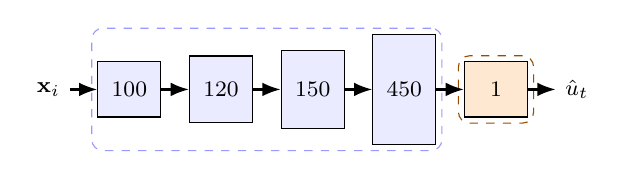
\begin{tikzpicture}[
    node distance=3.5mm,
    layer/.style={rectangle, draw, minimum height=8mm, minimum width=8mm,
                  font=\footnotesize, align=center},
    body/.style={layer, fill=blue!8},
    head/.style={layer, fill=orange!18},
    io/.style={font=\footnotesize, align=center},
    arrow/.style={-Latex, thick},
    label/.style={font=\scriptsize, align=center}
]
\node[io] (input) {$\mathbf{x}_i$};
\node[body, right=of input, minimum height=7mm] (b1) {100};
\node[body, right=of b1, minimum height=8.5mm] (b2) {120};
\node[body, right=of b2, minimum height=10mm] (b3) {150};
\node[body, right=of b3, minimum height=14mm] (b4) {450};
\node[head, right=of b4, minimum height=7mm] (head) {1};
\node[io, right=of head] (output) {$\hat{u}_t$};

\draw[arrow] (input) -- (b1);
\draw[arrow] (b1) -- (b2);
\draw[arrow] (b2) -- (b3);
\draw[arrow] (b3) -- (b4);
\draw[arrow] (b4) -- (head);
\draw[arrow] (head) -- (output);

\begin{scope}[on background layer]
  \node[draw=blue!40, dashed, rounded corners,
        fit=(b1)(b2)(b3)(b4),
        inner sep=2pt,
        label={[label, blue!60!black]above:Body (SiLU, meta-trained only)}]
       (bodybox) {};
  \node[draw=orange!60!black, dashed, rounded corners,
        fit=(head),
        inner sep=2pt,
        label={[label, orange!60!black]above:Head (adapts per task)}]
       (headbox) {};
\end{scope}
\end{tikzpicture}
\caption{Per-mixer architecture. Body: four-layer expanding SiLU MLP with
hidden widths $[100, 120, 150, 450]$; meta-trained only via outer Adam.
Head: linear projection $450 \to 1$; adapts per task via inner L-BFGS
under the ANIL split~\cite{raghu2020}. Paired PDEs (Brusselator,
$\lambda$-$\omega$) use two such mixers in parallel, one per output
equation.}
\label{fig:mixer_arch}
\end{figure}

\subsubsection{Inner Loop, Outer Loop, and Implicit Gradient}\label{subsubsec:imaml_math}

Formally, for task $\mathcal{T}_i$ with support set $\mathcal{D}_i^{\text{tr}}$ and
query set $\mathcal{D}_i^{\text{te}}$, per-task adaptation minimises the
proximal-regularised objective
\begin{equation}\label{eq:inner_objective}
G_i(\phi; \theta) =
    \mathcal{L}_i(\phi, \mathcal{D}_i^{\text{tr}})
    + \frac{\lambda}{2} \| \phi - \theta \|^2
\end{equation}
over $\phi$, where $\mathcal{L}_i$ is the per-mixer total loss
(\S\ref{subsubsec:loss_composition}) summed across mixers and $\lambda$
is the proximal coefficient. Inner optimisation runs L-BFGS for
$T = 60$ steps starting from $\phi := \theta$, updating only the head
under ANIL.

Let $\phi_i(\theta) := \text{Alg}(\theta, \mathcal{D}^{\text{tr}}_i)$ denote the resulting adapted parameters. The
meta-gradient is the gradient of the post-adaptation query loss with
respect to the meta-init:
\begin{equation}\label{eq:meta_gradient}
\nabla_\theta\,\mathcal{L}_i(\phi_i(\theta), \mathcal{D}_i^{\text{test}})
=
\left(\frac{d\phi_i}{d\theta}\right)^{\!\top}
\nabla_\phi\,\mathcal{L}_i(\phi_i(\theta), \mathcal{D}_i^{\text{test}}).
\end{equation}
By implicit differentiation of the inner-loop optimality condition
(Rajeswaran et al.~\cite{rajeswaran2019}, Lemma~1), the implicit
Jacobian is
\begin{equation}\label{eq:implicit_jacobian}
\frac{d\phi_i}{d\theta}
=
\left(I + \frac{1}{\lambda}
   \nabla^2_\phi\,\hat{\mathcal{L}}_i(\phi_i)\right)^{-1}.
\end{equation}
The matrix product in~\eqref{eq:meta_gradient} is never formed
explicitly; instead the linear system
\begin{equation}\label{eq:cg_system}
\left(I + \frac{1}{\lambda}
   \nabla^2_\phi\,\hat{\mathcal{L}}_i(\phi_i)\right) g_i = v_i,
\qquad
v_i := \nabla_\phi\,\mathcal{L}_i(\phi_i, \mathcal{D}_i^{\text{te}})
\end{equation}
is solved for $g_i$ by $J = 10$ iterations of conjugate
gradient~\cite{hestenes1952}, where $v_i$ is the partial
outer-level gradient and $g_i$ is the corrected per-task
meta-gradient.\footnote{For numerical stability, the implementation
follows the reference $\texttt{aravindr93/imaml\_dev}$
release~\cite{rajeswaran2019} and applies a damped variant of the
CG system, $\bigl((1+d_{\text{cg}})I + (\lambda+d_\lambda)^{-1}
\nabla^2\hat{\mathcal{L}}_i\bigr)\,g_i = v_i$, with $d_{\text{cg}} = 1$
and $d_\lambda = 10$. The paper-form
system~\eqref{eq:cg_system} is recovered at $d_{\text{cg}} = d_\lambda
= 0$. The damping does not change the implicit-gradient
identity~\eqref{eq:implicit_jacobian}; it stabilises the linear solve
under finite-precision arithmetic.}
The outer Adam step then takes the mean of $g_i$ across the meta-batch.

The proximal coefficient $\lambda$ does triple duty: it keeps inner
adaptation regularised against drift from $\theta$; it shifts the
Hessian by $\lambda I$ so that the system in~\eqref{eq:cg_system} is
positive-definite (provided $\lambda$ dominates the most negative
eigenvalue of $\nabla^2 \hat{\mathcal{L}}_i$), making CG convergence
guaranteed; and it controls the bias-variance trade-off in the
meta-gradient estimate via Theorem~1 of
Rajeswaran et al.~\cite{rajeswaran2019}.

\subsubsection{Algorithm}\label{subsubsec:algorithm}

Algorithm~\ref{alg:imaml} writes out the full meta-training loop. The
inner-loop L-BFGS step on line~9 operates on the proximal-regularised
objective $G_i$ and updates only the head parameters; the implicit-Jacobian
CG solve on line~12 produces the per-task corrected meta-gradient
$g_i$ from~\eqref{eq:cg_system}. The Kendall log-variances $\{s_k\}$
(\S\ref{subsubsec:loss_composition}) are updated alongside $\theta$ in
the outer step.

\begin{algorithm}[!t]
\renewcommand{\algorithmicrequire}{\textbf{Require:}}
\renewcommand{\algorithmicensure}{\textbf{Output:}}
\begin{algorithmic}[1]
\REQUIRE meta-train tasks $\{\mathcal{T}_i\}$; outer learning rate $\beta$;
         proximal coefficient $\lambda$; inner steps $T$; CG iterations $J$
\STATE Initialise $\theta$ and Kendall log-variances $\{s_k\}$
\WHILE{not converged}
  \STATE Sample meta-batch $\mathcal{B} \subset \{\mathcal{T}_i\}$
  \FORALL{$\mathcal{T}_i \in \mathcal{B}$}
    \STATE Sample $(\mathcal{D}_i^{\text{tr}}, \mathcal{D}_i^{\text{te}})$ from $\mathcal{T}_i$
    \STATE $\phi_i \leftarrow \theta$
    \FORALL{$t \in \{1, \ldots, T\}$}
	\STATE $G_i \leftarrow \mathcal{L}_i(\phi_i, \mathcal{D}_i^{\text{tr}}) + \frac{\lambda}{2}\,\|\phi_i - \theta\|^2$
      \STATE $\phi_i^{\text{head}} \leftarrow \text{LBFGS-step}(G_i)$
             \COMMENT{ANIL: body frozen}
    \ENDFOR
    \STATE $v_i \leftarrow \nabla_\phi\,\mathcal{L}_i(\phi_i, \mathcal{D}_i^{\text{te}})$
           \COMMENT{pre-correction outer-level gradient}
    \STATE Solve $(I + \lambda^{-1} \nabla^2_\phi\,\hat{\mathcal{L}}_i(\phi_i))\,g_i = v_i$
           for $g_i$ via $J$-iter CG
  \ENDFOR
  \STATE $\hat{\nabla} F(\theta) \leftarrow \frac{1}{|\mathcal{B}|} \sum_{\mathcal{T}_i \in \mathcal{B}} g_i$
  \STATE $\theta \leftarrow \text{Adam-step}(\theta, \hat{\nabla} F(\theta); \beta)$
         \COMMENT{$\theta$ spans body, head, and Kendall log-variances $\{s_k\}$; all updated jointly in one step}
\ENDWHILE
\STATE \textbf{return} $\theta^*$
\end{algorithmic}
\caption{iMAML meta-training with ANIL inner adaptation. After
Rajeswaran et al.~\cite{rajeswaran2019}; ANIL split per
Raghu et al.~\cite{raghu2020}.}
\label{alg:imaml}
\end{algorithm}

\subsubsection{Loss Composition}\label{subsubsec:loss_composition}

Each per-mixer loss $\mathcal{L}_i$ combines a main mean-squared-error
term against the time-derivative target with one or more
\emph{auxiliary} terms that supervise the mixer's input-Jacobian against
analytical Jacobian identities derived from the PDE. For example, in
Heat linear-input mode the target $u_t = D \nabla^2 u$ implies
$\partial u_t / \partial u_{xx} = D$ and
$\partial u_t / \partial u_{yy} = D$ at every collocation point; one
auxiliary regresses each Jacobian component against $D$. In NLHeat raw
mode the target $u_t = K(1{-}u)\nabla^2 u$ implies
$\partial u_t / \partial u_{xx} = K(1{-}u)$, with the regression target
now state-dependent.

All auxiliaries use the normalised mean-squared-error form
\begin{equation}\label{eq:aux_nmse}
L_{\text{aux}} = \frac{\frac{1}{N}\sum_{i=1}^N (q_i - t_i)^2}
                       {\frac{1}{N}\sum_{i=1}^N t_i^2},
\end{equation}
where $q_i$ is the network-derived quantity at collocation point $i$ (a
Jacobian partial computed via JVP, or a derived quantity such as the
PDE residual for the Brusselator $k_1$ recovery), $t_i$ is the
analytical target, and $N$ is the number of collocation points.
Normalisation by $\overline{t^2}$ makes the loss scale-invariant across
coefficients of differing magnitude. Table~\ref{tab:aux_losses} lists
the auxiliary count and recovery paths per (variant, mixer); full
equations per cell are documented alongside the project's source
material.

\begin{table*}[!t]
\centering
\caption{Auxiliary loss counts and recovery paths per (variant, mixer).
Subscripts after a coefficient name indicate the input-feature path the
auxiliary supervises (e.g.~$D_{u_{xx}}$ regresses
$\partial f / \partial u_{xx}$ against $D$). The asterisk on $k_1^{*}$
denotes recovery via the PDE residual rather than a single Jacobian
partial. Superscripts $(0), (1)$ denote per-mixer instances of the same
coefficient.}
\label{tab:aux_losses}
\small
\begin{tabular}{@{}llcl@{}}
\toprule
Variant & Mixer & \# aux & Recovery paths \\
\midrule
Heat linear-input & 0 & 2 & $D_{u_{xx}},\, D_{u_{yy}}$ \\
NLHeat linear-input & 0 & 1 & $K$ \\
NLHeat spatial-input & 0 & 3 & $K_{u_{xx}},\, K_{u_{yy}},\, K_{u}$ \\
BR linear-input & 0 & 3 & $D_u,\, k_2^{(0)},\, k_1^{*}$ \\
BR linear-input & 1 & 2 & $D_v,\, k_2^{(1)}$ \\
BR spatial-input & 0 & 4 & $D_{u_{xx}},\, D_{u_{yy}},\, k_2^{(0)},\, k_1^{*}$ \\
BR spatial-input & 1 & 3 & $D_{v_{xx}},\, D_{v_{yy}},\, k_2^{(1)}$ \\
$\lambda$-$\omega$ linear-input & 0 & 4 & $D_u,\, a^{(0)},\, c^{(0;u^2 v)},\, c^{(0;v^3)}$ \\
$\lambda$-$\omega$ linear-input & 1 & 4 & $D_v,\, a^{(1)},\, c^{(1;u^3)},\, c^{(1;u v^2)}$ \\
$\lambda$-$\omega$ spatial-input & 0 & 4 & $D_{u_{xx}},\, D_{u_{yy}},\, a^{(0)},\, c^{(0)}$ \\
$\lambda$-$\omega$ spatial-input & 1 & 4 & $D_{v_{xx}},\, D_{v_{yy}},\, c^{(1)},\, a^{(1)}$ \\
\bottomrule
\end{tabular}
\end{table*}

The main MSE and the auxiliaries are combined per mixer using Kendall
uncertainty weighting~\cite{kendall2018}. Each loss component
$L_k$ receives a learned scalar log-variance $s_k$, and the per-mixer
total is
\begin{equation}\label{eq:kendall_total}
\mathcal{L}_{\text{total}} =
\sum_k \left[
   \tfrac{1}{2}\, e^{-s_k}\, L_k
   + \tfrac{1}{2}\, s_k
\right],
\end{equation}
where the first term down-weights noisy or hard losses (effective
weight $\tfrac{1}{2} e^{-s_k}$) and the second term prevents
$s_k \to \infty$ (which would silence $L_k$ entirely). For numerical
stability, $s_k$ is parameterised as $\log \sigma^2$ rather than $\sigma$
directly, following the recommendation of
Kendall et al.~\cite{kendall2018}. The log-variances are
meta-parameters: they belong to the same outer-update slice as the body
and head, so the single Adam step on
Algorithm~\ref{alg:imaml}, line~15 updates $\theta$ and $\{s_k\}$
jointly using the meta-gradient
$\hat{\nabla} F(\theta)$. Like the body, $\{s_k\}$ are not touched by
the inner-loop L-BFGS solve. They are also held frozen at their
meta-trained values during evaluation, ensuring the meta-trained and
baseline branches see identical loss weighting.

\subsection{Evaluation Metrics}\label{subsec:evaluation_metrics}

\subsubsection{Sampling Protocol}\label{subsubsec:sampling_protocol}

For each test task $\mathcal{T}_i$, support and query collocation points
are sampled jointly: $K_{\text{shot}} = 4000$ support points and a query
set ($Q = 20\,000$ for scalar PDEs, $Q = 40\,000$ for paired PDEs) are
drawn together from a 2-dimensional Sobol quasi-random
sequence~\cite{wu2023} over the spatial domain, then split into
disjoint sets. Snapshot indices are sampled uniformly at random from the
51 available snapshots per task (one snapshot per collocation point).
Both meta-trained and baseline branches receive the \emph{same} support
and query draws within each task --- a fairness invariant ensuring the
comparison isolates the effect of $\theta^*$ versus random initialisation
rather than differing data.

Noise is applied at the Fourier-coefficient source: before features and
targets are evaluated at collocation points, the field's Fourier
coefficients are perturbed by additive Gaussian noise scaled to the
coefficient magnitude. This propagates correlated noise through the
field and its spatial derivatives, simulating the realistic case where
measurement noise on the field implies amplified noise on derived
quantities. The four evaluated noise levels are
$\sigma \in \{0,\, 0.01,\, 0.05,\, 0.10\}$.

Fine-tuning runs for $60$ inner-loop steps per task per noise level,
with main and auxiliary losses recorded at fixed steps $\{0, 60\}$ ---
step $0$ being the meta-initialisation $\theta^*$ before any adaptation,
step $60$ being the post-adaptation state.

\subsubsection{Coefficient Recovery}\label{subsubsec:coefficient_recovery}

Per-task coefficient recovery is performed at each fixed step by
extracting the network's input-Jacobian via JVP and matching the
per-point estimates against the analytical targets enumerated in
Table~\ref{tab:aux_losses}. For coefficients tied to a single
feature-target identity (Heat $D$, NLHeat $K$, $\lambda$-$\omega$
diffusion), recovery is the per-point estimate averaged over the
holdout grid. For coefficients tied to multiple features
(Brusselator $k_1$ via the PDE residual, $\lambda$-$\omega$ $a$ and $c$
via the tangled Jacobian identities of the raw mode), recovery uses
ordinary-least-squares regression of the network's Jacobian on the
analytical target structure, returning slope, intercept, and a
\emph{recovery} $R^2$ jointly --- the cross-task coherence of the
true-vs-recovered coefficient relationship, distinct from the per-task
\emph{feasibility} $R^2$ of \S\ref{subsec:approximation_theory}.

The win/loss decision between meta-trained and baseline branches uses
the \emph{product score} per (task, coefficient):
\begin{equation}\label{eq:product_score}
\text{score} = \texttt{pct\_error} \,\cdot\, (1 - R^2),
\end{equation}
where $\text{pct\_error}$ is the absolute relative error of the per-task
coefficient mean and $R^2$ is the coefficient of determination of the
recovery regression. The product penalises both inaccuracy (large
pct\_error) and incoherent fits (low $R^2$); the branch with the lower
score wins on that (task, coefficient) cell. Per-experiment, per-noise
counts aggregate the win decisions over the 27 test tasks for each
coefficient independently. Full per-experiment, per-noise breakdowns
are reported in \S\ref{sec:results}.

\subsubsection{Holdout NMSE}\label{subsubsec:holdout_nmse}

The per-mixer normalised mean-squared error on the holdout set is
\begin{equation}\label{eq:nmse}
\text{NMSE}_m =
\frac{\frac{1}{Q}\sum_{i=1}^{Q} (\hat{y}_{m,i} - y_{m,i})^2}
     {\frac{1}{Q}\sum_{i=1}^{Q} y_{m,i}^2},
\end{equation}
computed without gradient propagation on the disjoint $Q$-point
holdout grid for each mixer $m$ (FNO-style
normalisation~\cite{li2021fno}). The denominator
$\overline{y_m^2}$ makes NMSE scale-invariant across PDEs of differing
target magnitude: an NMSE of $10^{-3}$ on Brusselator (target std
${\sim}\,200$) and an NMSE of $10^{-3}$ on NLHeat (target std
${\sim}\,9$) represent the same proportional fit quality. Per-experiment
holdout-NMSE plateaus across input modes are the empirical basis of the
linearity-tax measurement reported in \S\ref{sec:results}.

\subsubsection{Per-Task feasibility $R^2$ Distribution}\label{subsubsec:r2_methodology}

Per-task linear-fit feasibility is measured separately from the iMAML
training and evaluation pipeline, on the same data but without
involving the trained networks. For each test task and each
$(\text{PDE},\, \text{mode},\, \text{mixer})$ cell:

\begin{enumerate}
\item Twenty resamples are drawn using the trainer's
      \texttt{get\_support\_query\_split} routine with $Q = 20\,000$
      (scalar PDEs) or $Q = 40\,000$ (paired PDEs); each resample uses
      a distinct seed for an independent draw of collocation points and
      snapshot indices.
\item For each resample, an ordinary-least-squares linear regression is
      fit from the per-mixer feature set to the per-mixer target with
      intercept; the coefficient of determination $R^2$ is recorded.
\item The 20 per-resample $R^2$ values for one task are summarised by
      mean, standard deviation, minimum, and maximum.
\item These four within-task summaries are then aggregated across the
      27 test tasks of the cell by their own mean, standard deviation,
      minimum, and maximum, producing a $4 \times 4$ outer-by-inner
      statistic grid per (PDE, mode, mixer).
\end{enumerate}

The two-stage aggregation separates within-task sampling noise from
across-task structural variation. Within-task sampling noise is small
under $20\,000$--$40\,000$ Sobol-sampled points (mean within-task
standard deviation under $0.06$ across all cells), so the dominant
signal in the outer aggregation is across-task variation in linear-fit
feasibility. 

\subsection{Experiment Grid}\label{subsec:experiment_grid}

The main experimental grid is seven cells over the Cartesian product of
PDE family and input-feature mode, all sharing the iMAML training
protocol of \S\ref{subsec:meta_training_imaml} and the per-mixer
architecture of \S\ref{subsubsec:architecture}. The shared specification
is enumerated in Table~\ref{tab:shared_hyperparameters}; the
per-experiment differing axes (PDE, input mode, query size) are listed
in Table~\ref{tab:experiment_grid}.

\begin{table}[!t]
\centering
\caption{Shared hyperparameters across all seven main experiments}
\label{tab:shared_hyperparameters}
\small
\begin{tabular}{@{}ll@{}}
\toprule
Parameter & Value \\
\midrule
\multicolumn{2}{@{}l}{\textit{Architecture}} \\
hidden dimensions     & $[100, 120, 150, 450]$ \\
activation            & SiLU \\
ANIL inner-adapt slice & head-only \\
\midrule
\multicolumn{2}{@{}l}{\textit{Inner loop}} \\
optimizer             & L-BFGS \\
inner steps $T$       & 60 \\
proximal $\lambda$    & $5\times 10^{-3}$ \\
\midrule
\multicolumn{2}{@{}l}{\textit{Outer loop}} \\
optimizer             & Adam \\
$(\beta_1, \beta_2)$  & $(0.9,\, 0.999)$ \\
outer LR $\beta$      & $3.5\times 10^{-3}$ \\
LR schedule           & polynomial, $p = 3$ \\
schedule $T_0, T_{\text{mult}}$ & $200,\, 2$ \\
$\text{min\_lr}$      & $10^{-7}$ \\
gradient clip norm    & $10.0$ \\
meta-batch size       & 28 \\
max iterations        & 2000 \\
\midrule
\multicolumn{2}{@{}l}{\textit{Implicit gradient}} \\
CG iterations $J$     & 10 \\
CG damping $d_{\text{cg}}$ & $1.0$ \\
$\lambda$-damping $d_\lambda$ & $10.0$ \\
\midrule
\multicolumn{2}{@{}l}{\textit{Data}} \\
support size $K_{\text{shot}}$ & 4000 \\
loss function         & normalised MSE \\
\bottomrule
\end{tabular}
\end{table}

\begin{table}[!t]
\centering
\caption{Differing axes across the seven main experiments. Mode
abbreviations match \S\ref{subsubsec:input_feature_modes}: \emph{library}
and \emph{linear-input} are linear-input variants, \emph{raw} is the
spatial-input variant. Query size $Q$ scales with mixer count.}
\label{tab:experiment_grid}
\small
\begin{tabular}{@{}lllc@{}}
\toprule
Experiment                  & PDE   & Mode       & $Q$    \\
\midrule
heat-60step                 & Heat  & linear-input& 20\,000 \\
nl\_heat-60step             & NLHeat & linear-input & 20\,000 \\
nl\_heat-60step-raw         & NLHeat & spatial-input& 20\,000 \\
br-60step                   & BR    & linear-input & 40\,000 \\
br-60step-raw               & BR    & spatial-input & 40\,000 \\
lo-60step                   & LO    & linear-input & 40\,000 \\
lo-60step-raw               & LO    & spatial-input & 40\,000 \\
\bottomrule
\end{tabular}
\end{table}

\subsection{Testing and Development}\label{subsec:testing_dev}

Two parts of the pipeline used \emph{oracle} access to ground-truth per-task
PDE coefficients. The Jacobian-identity auxiliary losses of
\S\ref{subsubsec:loss_composition} regress the network's input-Jacobian
against analytical targets computed from the per-task coefficient values
used in Dedalus generation, and the coefficient recovery routine of
\S\ref{subsubsec:coefficient_recovery} scores the Jacobian-extracted
estimates against those same oracle values. The work is therefore
amortisation conditioned on a known equation form and known coefficients
at training and evaluation, not blind discovery in the SINDy sense; the
deliverables argue inside that regime.

Several development hurdles surfaced. CG inverse-Hessian solves are
ill-conditioned in finite precision and required the damped variant
($d_{\text{cg}}{=}1.0$, $d_\lambda{=}10.0$) of the
\texttt{aravindr93/imaml\_dev} release. OLS for the per-task linear-fit
feasibility runs on CPU through \texttt{torch.linalg.pinv} because CUDA
\texttt{lstsq} returns NaN on certain ill-conditioned $\lambda$-$\omega$
raw feature matrices. ANIL's body--head split is load-bearing: without
it, inner-loop L-BFGS overfits the support set within a few steps and
the meta-gradient signal collapses. Linear-input modes attaining
in-sample $R^2 = 1.000$ across all four PDE families acts as a
continuous sanity check on data generation: by analytical construction
the target is a linear combination of the supplied features under the
task-specific coefficients, so any drop below unity flags pipeline drift
before any meta-training is run.

\section{Results}\label{sec:results}

\subsection{Per-Coefficient Recovery}\label{subsec:results_coeff_recovery}

Table~\ref{tab:coeff_recovery_full} reports the per-coefficient mean
recovery error across 27 test tasks for each
(experiment, coefficient, noise) cell. Each (experiment, coefficient)
block carries two stacked rows: the meta-trained branch (MAML) on top
and the baseline branch (BL) below. Each cell reads as
``mean$\,\pm\,$std $[\min,\,\max]$'' inline. Bold marks the row's
winner per noise column, decided by per-task win count under the
product score of \eqref{eq:product_score}. Both methods report on the
same support and query draws within each task
(\S\ref{subsubsec:sampling_protocol}). The table is presented in
landscape orientation (\texttt{sidewaystable*}) for legibility at
the four-statistic-per-cell density.

\input{tables/coefficient_recovery}

Table~\ref{tab:coeff_recovery_r2} reports the parallel \emph{recovery}
$R^2$ for the same per-task coefficient-recovery regressions. Cells
use the same inline format and the same per-noise winner bolding as
Table~\ref{tab:coeff_recovery_full}; the winner is determined by the
shared product score, so the bold pattern matches across the two
tables --- the $R^2$ table reveals when a winning method's coefficient
estimate is also \emph{coherent} (high $R^2$) versus merely on average
correct (low $R^2$).

\input{tables/coefficient_recovery_r2}

\subsection{Holdout-NMSE Win Rate}\label{subsec:results_nmse_wins}

Table~\ref{tab:nmse_wins} aggregates per-mixer holdout-NMSE win counts
across the seven main experiments, summed over 27 tasks $\times$
4 noise levels (108 cells per experiment). A win is defined as the
meta-trained branch achieving lower per-mixer-summed NMSE on the
holdout grid; the count therefore measures how often the meta-init
beats a random init at per-task fit quality.

\begin{table}[!t]
\centering
\caption{Per-experiment holdout-NMSE win counts, summed over 27 tasks
$\times$ 4 noise levels (108 cells per experiment).}
\label{tab:nmse_wins}
\scriptsize
\begin{tabular}{@{}lrr@{}}
\toprule
Experiment                    & Wins / 108 & Win rate \\
\midrule
heat-60step                   & 16  & 14.815\,\% \\
nl\_heat-60step               & 27  & 25.000\,\% \\
nl\_heat-60step-raw           & 67  & 62.037\,\% \\
br-60step                     & 95  & 87.963\,\% \\
br-60step-raw                 & 107 & 99.074\,\% \\
lo-60step                     & 90  & 83.333\,\% \\
lo-60step-raw                 & 108 & 100.000\,\% \\
\bottomrule
\end{tabular}
\end{table}

\subsection{Linear Decodability and Linearity Tax}\label{subsec:results_linearity_tax}

Table~\ref{tab:per_task_r2} reports the resampling-based per-task
$R^2$ statistics over 27 test tasks $\times$ 20 resamples per cell.
For each cell, the inner mean / std / min / max are first computed
within each task across the 20 resamples; the four outer columns then
aggregate the per-task means across the 27 tasks of the cell.

\begin{table*}[!t]
\centering
\caption{Per-task linear-fit feasibility $R^2$ across 27 test tasks
$\times$ 20 resamples per (PDE, mode, mixer) cell. Columns report the
distribution of per-task means across the 27 tasks. All linear-input
modes (Heat library, NLHeat library, BR library, LO library)
attain per-task $R^2 = 1.000$ with zero across-task variance.}
\label{tab:per_task_r2}
\small
\begin{tabular}{@{}lrrrr@{}}
\toprule
Cell                  & mean(mean) & std(mean) & min(mean) & max(mean) \\
\midrule
Heat library          & 1.000 & 0.000 & 1.000 & 1.000 \\
NLHeat library		  & 1.000 & 0.000 & 1.000 & 1.000 \\
NLHeat raw            & 0.731 & 0.263 & 0.171 & 0.994 \\
BR library m0         & 1.000 & 0.000 & 1.000 & 1.000 \\
BR library m1         & 1.000 & 0.000 & 1.000 & 1.000 \\
BR raw m0             & 0.973 & 0.056 & 0.808 & 1.000 \\
BR raw m1             & 0.964 & 0.096 & 0.584 & 1.000 \\
LO library m0         & 1.000 & 0.000 & 1.000 & 1.000 \\
LO library m1         & 1.000 & 0.000 & 1.000 & 1.000 \\
LO raw m0             & 0.983 & 0.017 & 0.929 & 1.000 \\
LO raw m1             & 0.982 & 0.021 & 0.930 & 1.000 \\
\bottomrule
\end{tabular}
\end{table*}

Table~\ref{tab:linearity_tax} reports the linearity tax per PDE: the
ratio of the spatial-input mode's NMSE plateau to the linear-input
mode's NMSE plateau, computed at meta-training iteration 1999 with a
50-iter trailing window. Higher ratio indicates a larger gap between
the network's convergence floor under the two feature designs --- the
tax measurement of \S\ref{subsec:approximation_theory}. Heat is
omitted: it has no spatial-input variant
(\S\ref{subsubsec:input_feature_modes}).

\begin{table}[!t]
\centering
\caption{Linearity tax per PDE / mixer. Plateaus are 50-iter trailing
means at iter 1999 of \texttt{mse\_main} from each experiment's
training history.}
\label{tab:linearity_tax}
\small
\begin{tabular}{@{}lrrr@{}}
\toprule
PDE / mixer    & linear-input         & spatial-input        & ratio                \\
\midrule
NLHeat         & $1.60\times 10^{-6}$ & $1.03\times 10^{-3}$ & $\mathbf{642\times}$ \\
BR (mixer 0)   & $2.69\times 10^{-6}$ & $6.55\times 10^{-5}$ & $\mathbf{24\times}$  \\
BR (mixer 1)   & $1.50\times 10^{-5}$ & $9.26\times 10^{-5}$ & $6\times$            \\
LO (mixer 0)   & $8.00\times 10^{-6}$ & $1.25\times 10^{-5}$ & $\mathbf{1.6\times}$ \\
LO (mixer 1)   & $7.58\times 10^{-6}$ & $1.97\times 10^{-5}$ & $2.6\times$          \\
\bottomrule
\end{tabular}
\end{table}

Figure~\ref{fig:tax_ratio} plots the same spatial-input/linear-input
ratio across the entire meta-training trajectory for each PDE-mixer
pair. The y-axis is on a log scale; the dotted reference line at
$\text{ratio} = 1$ marks parity between modes. Following an
early-training transient, all three PDEs settle into stable plateaus
that match the iteration-1999 values reported in
Table~\ref{tab:linearity_tax}.

\begin{figure}[!t]
\centering
\includegraphics[width=\linewidth]{training_loss_ratios.png}
\caption{Spatial-input/linear-input \texttt{mse\_main} ratio across
meta-training iterations, per PDE and per mixer; y-axis is log-scaled.
NLHeat (top-left) plateaus near $600\times$; BR (top-right) plateaus
near $24\times$ on mixer 0 and $6\times$ on mixer 1;
$\lambda$-$\omega$ (bottom) plateaus near $1.6\times$ on mixer 0 and
$2.6\times$ on mixer 1.}
\label{fig:tax_ratio}
\end{figure}

\section{Evaluation}\label{sec:evaluation}

% TODO(voice) -- academic preamble:
%   "This section interprets ... along three axes" is template framing. Skip
%   the preview; lead with the analytical claim. Headers announce themselves.

The relation between coefficient recovery \texttt{error\_pct} and recovery coherence $R^2$
(\S\ref{subsec:eval_headline_mechanism}); the occurrence of the feature
linearity tax phenomena (\S\ref{subsec:eval_linearity_tax}); and the boundary
at which meta-initialisation ceases to outperform random initialisation
(\S\ref{subsec:eval_value_boundary}), will be explained with empirical
backing.

\subsection{Recovery versus Coherence}\label{subsec:eval_headline_mechanism}

% TODO(voice) -- procedural setup:
%   "Tables N and M bold each cell..." reads as third-party. Your voice would
%   lead with the claim ("Recovery and coherence decouple in two regimes")
%   then anchor in the bolding rule.


Tables~\ref{tab:coeff_recovery_full} and~\ref{tab:coeff_recovery_r2} bold each
cell independently on its own metric: the pct\_error table bolds the row with
the lower per-task win count under product score; the recovery $R^2$ table
bolds the row with the higher $R^2$ mean. A cell emphasised in
Table~\ref{tab:coeff_recovery_full} means the center of its learnt
distribution of predictions is more precise and accurate relative to the
Baseline's convergence, ensuring that each task is won accuracy-wise as well.
Where the two tables agree on bolding, the meta-trained and baseline rankings on
coefficient accuracy and on Jacobian coherence coincide. Where the two tables
disagree, the metrics diverge --- one method is winning on mean coefficient
accuracy while the other is winning on the underlying linear fit's coherence.
The \texttt{pct\_error} table answers whether the meta-trained branch's
coefficient estimate is closer to the true value on average; the $R^2$ table
answers whether the underlying Jacobian regression is \emph{coherent}, with
per-point estimates clustering around a consistent slope rather than
scattering.

% TODO(voice) -- observer phrasing:
%   "The two tables agree on the easy regimes" is detached. Your voice would
%   commit: "Heat and NLHeat are the trivial regime --- both methods solve
%   it; the bold is between two coherent recoveries."
The two tables agree on the easy regimes. heat-60step and
nl\_heat-60step sit in baseline-wins-by-tiebreaker territory: both
methods reach $R^2 \geq 0.99$ across noise levels, mean errors below
$0.1\,\%$, and the baseline edges out by tiny margins. In these
cells the bold marker selects between two coherent recoveries that
both essentially solve the problem.

% TODO(voice) -- measured-observer:
%   "The tables diverge ... reading X alongside reveals" is my measured
%   register. Your voice would name it as an argument: "NLHeat-raw at
%   sigma=0.10 is two failures, not a winner-loser."
The tables diverge on the hard regimes. nl\_heat-60step-raw at
$\sigma{=}0.10$ has the meta-trained branch at $6.806\,\%$ mean error
and $R^2$ mean $-0.183$ (range $[-1.366,\,0.117]$), while the baseline
reaches $4.553\,\%$ mean error and $R^2$ mean $-8.231$ (range
$[-30.739,\,0.003]$). The baseline's lower mean error is bolded,
selected by product score because the baseline's $R^2$ collapse,
though more catastrophic in absolute terms, still pairs with a
smaller per-task mean error. The \texttt{pct\_error} table read alone makes
this look like a clean baseline win at high noise; reading
Table~\ref{tab:coeff_recovery_r2} alongside reveals that neither
method has a coherent linear fit at this noise level, so the
``contest'' is between two failures rather than a winner and a loser. And this
can be observed recurringly.

% TODO(voice) -- third-party closing:
%   "X maintains coherent recovery; the baseline does not" is observer-style
%   close. Attach this to the lo-raw vs lo-library narrative from your
%   earlier analysis (lo-raw recovery R^2 stays at 1.0, baseline coefficient
%   mean wanders far on c).
The recovery $R^2$ evidence sharpens elsewhere too. lo-60step-raw at
$\sigma{=}0.05$ has meta-trained $R^2$ at $1.000\,\pm\,0.000$ across
all four coefficients while baseline drops to $0.998\,\pm\,0.001$.
The narrow $R^2$ gap is consistent with the baseline's catastrophic
\texttt{pct\_error} blow-up on $c$ at this cell ($27.345\,\%$ mean error vs the
meta-trained branch's $2.697\,\%$): the baseline's coefficient mean
wanders far from truth even when the underlying linear-fit residuals
look small per-task. The meta-trained branch maintains coherent
recovery here; the baseline does not.

\subsection{Linearity Tax Structure}\label{subsec:eval_linearity_tax}

% TODO(voice) -- academic-summary register:
%   "Plateau ratios ... span two orders of magnitude ... co-monotones with
%   ... consistent with linear decodability acting as a structural
%   component" is mine. Your voice argues that the NLHeat/BR/LO tax
%   ordering is preordained by feature design --- feasibility R^2 fixes the
%   structural floor.
The plateau ratios in Table~\ref{tab:linearity_tax} span two orders of
magnitude across the three PDE families, in the ordering 

\begin{align*}
\mathbf{nl\_heat} (642\times) &\gg \mathbf{BR} (24\times \text{ on mixer 0}) \\
&> \mathbf{LO} (1.6\times \text{ on mixer 0}).
\end{align*}
Upon looking at the individual model performances, there is an occurrence to be
observed, such that when you rank Table 10 by ascending order of the column
$\mathbf{mean}(\text{mean}) \times \mathbf{std}(\text{mean})$ you get Table 12.

\begin{table}[!t]
\centering
\caption{Co-ordering of spatial-input cells by
feasibility-distribution complexity (left, from
Table~\ref{tab:per_task_r2}) and by absolute spatial-input plateau
loss (right, from Table~\ref{tab:linearity_tax}). Both rankings give
the same ascending chain.}
\label{tab:tax_co_ordering}
\small
\begin{tabular}{@{}ll@{}}
\toprule
$\text{mean(mean)}\times\text{std(mean)}$ & Spatial-input plateau loss \\
\midrule
LO-raw-0 ($0.017$)        & LO-raw-0 ($1.25{\times}10^{-5}$) \\
LO-raw-1 ($0.021$)        & LO-raw-1 ($1.97{\times}10^{-5}$) \\
BR-raw-0 ($0.054$)        & BR-raw-0 ($6.55{\times}10^{-5}$) \\
BR-raw-1 ($0.093$)        & BR-raw-1 ($9.26{\times}10^{-5}$) \\
NLHeat-raw ($0.192$)      & NLHeat-raw ($1.03{\times}10^{-3}$) \\
\bottomrule
\end{tabular}
\end{table}

The NMSE holdout metric had provided bound floor loss that correlates with the
product $\mathbf{mean}(\text{mean}) \times \mathbf{std}(\text{mean})$.
Minimising this \emph{implies} minimising variance of the mean of aggregated per-task
$R^2$. In this construction it's not likely for $\mathbf{mean}(\text{mean})$ to
approach $0$ and have $\mathbf{mean}(\text{mean})\times\mathbf{std}(\text{mean})
\to 0$, as by then, $\mathbf{std}(\text{mean})$ will rise by reaction. NLHeat raw
having the highest score entails that the SiLU model has to interpolate more
effectively across untight regressions. The product in essence measures the
tightness of its aggregated linear explanations per-task-sampled $R^2(\vec{x}|\hat{y})$, 
where $\vec{x}$ is a vector containing all features.

This argues that \emph{linear-input} feature mode guarantees convergence
because high linear decodability on the task distribution empirically shows
lower loss floors. Presumably, the floor of the tax is observed not by
feasibility mean alone but by mean and within-task spread jointly: a cell whose
feasibility is high on average but distributes non-trivial spread per task pays
an absolute floor different from one whose feasibility is uniformly tighter,
and the SiLU MLP's spatial-input plateau tracks the joint quantity rather than
either component in isolation.

Given by the stats of NLHeat raw, there pertain more tasks than
usual that cannot be linearly explained. This occurrence then shows negative
effects on the optimisation trajectory, adding more noise, and oscillations in
Figure~\ref{fig:training_loss}.

\begin{figure*}[!t]
\centering
\includegraphics[width=\textwidth]{training_loss_main_aux.png}
\caption{Per-experiment training loss trajectories: main MSE plus
auxiliary Jacobian-identity losses across meta-training iterations,
per PDE family and per mixer. NLHeat-raw's high-amplitude
oscillation is visible against the smoother descent of linear-input
modes.}
\label{fig:training_loss}
\end{figure*}


% TODO(voice) -- academic-formal:
%   "Provides a second sculpting axis" + "Following the constraint-
%   restriction reading" is mine. Your prior analysis already has it:
%   NLHeat raw had inadequate K aux loss design; rerunning with three
%   Jacobian paths closed the gap from 2231x to 642x. Lift that argument.

Notably, ablations with auxiliary-loss design suggest that optimisation functions also
affect the floor of the meta-training loss. Before, \texttt{nl\_heat-60steps-raw} model had been
setup to be trained with 2 aux loss functions, that probes for K coefficient
learning in two distinct paths: $u_{xx}$-path $K_{u_{xx}}$ and $u_{yy}$-path
$K_{u_{yy}}$. \texttt{nl\_heat-60step-raw} was retrained with three Jacobian-identity
supervision paths --- the third regressing $\partial f_\theta / \partial u$
against $-K(u_{xx}+u_{yy})$, complementing the two Laplacian-component paths of
the earlier configuration. Win rate on holdout NMSE rose from $48.1\,\%$ to
$62.0\,\%$, and the linearity-tax ratio dropped from a previous $2231\times$ at
iteration 1999 to the current $642\times$. Following the constraint-restriction
reading of Liebel and K\"orner~\cite{liebel2018}, each additional aux path
narrows the admissible parameter region by adding a regression constraint on
the network's input-Jacobian. The empirical effect suggests that
aux-supervision adequacy is a sculpting axis independent of feature-mode choice
and merits separate treatment when comparing tax magnitudes across experiments.

% TODO(voice) -- figure-reference template:
%   "Figure X gives the temporal complement of Table Y" is template phrasing.
%   Compress: "The tax is reached after the early-training transient
%   (~250 iter) and persists --- not transient on the way to parity."
Figure~\ref{fig:tax_ratio} gives the temporal complement of
Table~\ref{tab:linearity_tax}. All three PDEs settle into stable
plateaus after the early-training transient ($\lesssim 250$
iterations), with the plateau values matching the iteration-1999
numbers reported in the table. The tax is a persistent property of
the meta-trained model under the present setup, not a transient on
the way to parity.

\subsection{The Boundary of Meta-Learning's Value}\label{subsec:eval_value_boundary}

% TODO(voice) -- list-then-claim:
%   "Table X reports ... in the order [list] ... ordering is monotone with
%   structural difficulty" leads with data. Your voice would lead with the
%   claim ("MAML wins more as the problem gets harder for both methods")
%   then drop the list.
Table~\ref{tab:nmse_wins} reports holdout-NMSE win rates in the order
heat-60step $14.8\,\%$, nl\_heat-60step $25.0\,\%$,
nl\_heat-60step-raw $62.0\,\%$, br-60step $88.0\,\%$,
br-60step-raw $99.1\,\%$, lo-60step $83.3\,\%$,
lo-60step-raw $100\,\%$. The ordering is monotone with structural
difficulty: meta-initialisation wins more often as the problem
becomes harder for both methods. The two endpoints --- heat-60step
at $14.8\,\%$ and lo-60step-raw at $100\,\%$ --- bracket the regime
in which meta-learning's prior is meaningful.

% TODO(voice) -- bias-variance academic register (HEAVIEST SEAM):
%   "The bias-variance reading is that ..." is the most clearly mine
%   paragraph in the report. Your voice argues from system structure:
%   "This argues that implicit-wise mixings on linear-input mode is too
%   cheap a class for amortisation to pay off. Baseline reaches the
%   per-task fit in 60 L-BFGS from random init; MAML's prior is on the
%   cost side, not the value side, at sigma <= 0.01."
Per-coefficient inspection (Table~\ref{tab:coeff_recovery_full})
sharpens the boundary. Even on PDEs where the meta-trained branch
wins overall, specific cells at $\sigma{=}0.01$ in linear-input mode
go to baseline: all four LO library coefficients
($D_u,\,D_v,\,a,\,c$) show baseline-bold cells at this noise level.
The bias-variance reading is that baseline's full-network adaptation
reaches a per-task linear-feature fit fast enough that 60 L-BFGS
steps from random initialisation arrive at the same near-convex
minimum the meta-learned $\theta^*$ occupies; the prior that helps
on harder problems is then a slight pull-off-optimum on trivial
ones. The pattern reproduces across heat-60step, nl\_heat-60step,
and lo-60step --- three PDE families, all in linear-input mode at
$\sigma \leq 0.01$.

% TODO(voice) -- observer summary:
%   "The boundary lies between sigma=0.01 and sigma=0.05" + "becomes a
%   noise-fitting liability" is observer. Your voice commits: "Above
%   sigma=0.05 the picture flips. Cross-PDE reproducibility argues this is
%   structural-target-linearity x noise level, not PDE-specific."
The boundary lies between $\sigma{=}0.01$ and $\sigma{=}0.05$ on
linear-input experiments. Above this regime, baseline's full
parameter capacity becomes a noise-fitting liability; the
meta-trained branch's head-only ANIL adaptation has fewer parameters
available to overfit and degrades more gracefully. The cross-PDE
reproducibility of the regime suggests it depends on
linear decodability and noise level rather than on
PDE-specific properties.

\subsection{Self-Assessment}\label{subsec:eval_self_assess}

The strongest part of this work is that the empirical observations were
at least explained with backing from the existing literature. The
linear-decodability framing of \S\ref{subsubsec:feature_distribution}
(Alain and Bengio, Bengio et al., Tancik et al.,
Wang-Wang-Perdikaris), the Sobolev-training argument for SiLU
(Czarnecki et al.), and the constraint-restriction reading of multi-task
auxiliaries (Liebel and K\"orner) provided structural anchoring for what
would otherwise be standalone observations.

A1 could have done more. More theoretical work, proofs, and orthogonal
ablations on the linearity-tax argument would have sharpened the
empirical co-ordering of Table~\ref{tab:tax_co_ordering} into a
structural claim rather than a measurement. The per-task linear-fit
feasibility $R^2$ diagnostic of \S\ref{subsubsec:r2_methodology} only
emerged late in the project timeline; the follow-through on it was not
afforded. Deliverables B1--B3, I1--I2, and A1 themselves ran to
completion across the seven main experiments and four noise levels,
returning the win-rate ordering of Table~\ref{tab:nmse_wins}.

\section{Conclusion}\label{sec:conclusion}

% TODO(voice) -- abstract-style opening:
%   "Input-feature design materially modulates the convergence floor" is
%   abstract-summary register. Your voice opens conclusion with the
%   argumentative thread that ties feasibility-R^2 ordering, linearity-tax
%   ordering, and win-rate ordering into one "this argues that ..." chain.
Input-feature design representationally modulates the convergence floor of
meta-learned PDE coefficient discovery: linear-input modes admit
per-task linear-fit feasibility $R^2 = 1.000$ across four PDE
families, while spatial-input modes carry a linearity tax ranging
from $1.6\times$ ($\lambda$-$\omega$) to $642\times$ (NLHeat) according
to the linear decodability of the target. The questions
investigated were whether iMAML over PDE coefficient distributions
can produce an amortisation effect on PDE coefficient recovery
against a from-scratch randomly initialised baseline, and how the
choice of input-feature design --- \emph{linear-input} versus
\emph{spatial-input} --- reshapes the quality of that amortisation.
Deliverables B1--B3 (pipeline plus Heat amortisation), I1--I2
(NLHeat, Brusselator, $\lambda$-$\omega$ amortisations), and A1 (the
linear-input vs spatial-input ablation) were all delivered.

% TODO(voice) -- enumeration template:
%   "The empirical findings are three. First, ... Second, ... Third, ..."
%   is academic-template. Your voice weaves the three findings into a
%   single argumentative paragraph using your coined ontology
%   (implicit-wise / cross-input-wise / residual-wise mixings) where it
%   applies. Don't enumerate; argue.
It is suggestive that FFN neural networks have this strong affinity to data
distributions of high linear decodability. Unfortunately, the empirical
evidence here is still not enough to ground such claim and need further
ablations and theoretical work. What is worth showing nonetheless is the effect
of input feature design on optimisation in which we can measure it with an
approach of aggregating feasibility for $R^2$. It is through per-sampling
linear-fit $R^2$ probing that the gap between linear-input and spatial-input
feature modes is empirically made measurable. Linear-input cells uniformly
attain $R^2 = 1.000$ across all four PDE families with zero across-task
variance, while spatial-input cells distribute non-trivial spread per task.
This argues that linear-input is much more usable than spatial-input. Turning
into linear-input feature mode allows the model to directly learn the
coefficients with straightforward jacobian probing as each coefficient can have
its input feature designed to even disentangle two coefficients in one term.

With the monotonic increase of the holdout-NMSE winrate $14.8\%$
(\texttt{heat-60step}, where both methods solve the problem trivially, but with
MAML prior causing its deficit) to $100\%$ (\texttt{lo-60step-raw}, where the
meta-learned prior bridges a structural optimisation gap that random
initialisation cannot close in 60 inner steps), unlike
\texttt{nl\_heat-60step-raw}, two experiments \texttt{br-60step-raw} and
\texttt{lo-60step-raw} were able to relatively catch up to their
\emph{linear-input} counterparts. And this is explained by per-task sampling
linear-fit $R^2$, aggregated across tasks which has
\texttt{nl\_heat-60step-raw} showing the lowest and most spread out samples
$\{R^2\}$. Given that \texttt{nl\_heat-60step-raw} is shown to be the most
challenging PDE for both MAML and Baseline models, MAML was able to dominate
wins on Baseline. This is evidence of amortisation.

% TODO(voice) -- enumeration template:
%   "The methodological contributions are two. First, ... Second, ..." is
%   template. Frame these as natural consequences of the system rather than
%   numbered contributions.
The appropriation of per-task linear-fit feasibility, the
ordinary-least-squares $R^2$ of the target on the mode's feature set, measured
by resampling per test task, served as a diagnostic for PDE feature designs,
enacting as the regression analogue of the probe-classifier technique of Alain
and Bengio~\cite{alain2017} applied to the linear-decodability question of
\S\ref{subsec:approximation_theory}. Second, the adequacy of the
Jacobian-identity auxiliary-loss design acts as a sculpting axis on the
parameter manifold independent of input-mode choice: NLHeat-raw with three
Jacobian-recovery paths attains a $642\times$ tax versus the previous two-path
configuration's $2231\times$ at the same feature mode, supporting the
constraint-restriction reading of multi-task auxiliaries (Liebel and
K\"orner~\cite{liebel2018}).

% TODO(voice) -- academic future-work:
%   "Several questions remain open ... Two extensions are concrete enough
%   to be worth flagging" is template. Your voice opens questions as
%   ongoing tensions, e.g. "k1 residual-wise mixer presence is an open
%   question."
Lastly, several questions remain open. The linear-target low-noise baseline
advantage of \S\ref{subsec:eval_value_boundary} was probed empirically on
$\lambda$-$\omega$ library; cross-PDE generalisation to Heat and NLHeat-60step
is consistent with the bias-variance reading but not directly verified through
loss-landscape probes. Two extensions are concrete enough to be worth flagging.
\emph{Mixed-noise meta-training}, in which the noise level $\sigma$ is drawn
per task from a range during meta-training rather than held at zero, would test
whether the meta-trained branch's deficit at $\sigma \leq 0.01$ on linear-input
modes is a property of clean-only meta-training that disappears under noise
exposure. \emph{Cross-architecture extension} would be probing the learned
mapping of an FFN block's latent input to its latent output, embedded within a
larger transformer or convolutional architecture. The ablation itself is just
per-task $R^2$ on the full latent input features against the FFN block's
output, testing whether the loss floor of the whole large architecture is
predicted the same way as the SiLU MLP body's floor of this work.


% trigger a \newpage just before the given reference
% number - used to balance the columns on the last page
% adjust value as needed - may need to be readjusted if
% the document is modified later
%\IEEEtriggeratref{8}
% The "triggered" command can be changed if desired:
%\IEEEtriggercmd{\enlargethispage{-5in}}

% references section

% can use a bibliography generated by BibTeX as a .bbl file
% BibTeX documentation can be easily obtained at:
% http://mirror.ctan.org/biblio/bibtex/contrib/doc/
% The IEEEtran BibTeX style support page is at:
% http://www.michaelshell.org/tex/ieeetran/bibtex/
%\bibliographystyle{IEEEtran}
% argument is your BibTeX string definitions and bibliography database(s)
%\bibliography{IEEEabrv,../bib/paper}
%
% <OR> manually copy in the resultant .bbl file
% set second argument of \begin to the number of references
% (used to reserve space for the reference number labels box)

\newpage
\begin{thebibliography}{99}

% --- Parent papers ---

\bibitem{raissi2018}
M.~Raissi, ``Deep Hidden Physics Models: Deep Learning of Nonlinear Partial
Differential Equations,'' \emph{Journal of Machine Learning Research},
vol.~19, no.~25, pp.~1--24, 2018.

\bibitem{raissi_code}
M.~Raissi, ``DeepHPMs: Deep learning of nonlinear partial differential
equations,'' GitHub repository, 2018. [Online]. Available:
\url{https://github.com/maziarraissi/DeepHPMs}

\bibitem{raissi2019pinn}
M.~Raissi, P.~Perdikaris, and G.~E. Karniadakis, ``Physics-informed neural
networks: A deep learning framework for solving forward and inverse problems
involving nonlinear partial differential equations,''
\emph{Journal of Computational Physics}, vol.~378, pp.~686--707, 2019.

\bibitem{finn2017}
C.~Finn, P.~Abbeel, and S.~Levine, ``Model-Agnostic Meta-Learning for Fast
Adaptation of Deep Networks,'' in \emph{Proc. 34th Int. Conf. Machine
Learning (ICML)}, ser. Proceedings of Machine Learning Research, vol.~70,
2017, pp.~1126--1135.

\bibitem{rajeswaran2019}
A.~Rajeswaran, C.~Finn, S.~M. Kakade, and S.~Levine, ``Meta-Learning with
Implicit Gradients,'' in \emph{Advances in Neural Information Processing
Systems (NeurIPS)}, vol.~32, 2019.

% --- Meta-learning literature ---

\bibitem{nichol2018}
A.~Nichol, J.~Achiam, and J.~Schulman, ``On First-Order Meta-Learning
Algorithms,'' arXiv preprint arXiv:1803.02999, 2018.

\bibitem{antoniou2019}
A.~Antoniou, H.~Edwards, and A.~Storkey, ``How to Train Your MAML,'' in
\emph{Int. Conf. Learning Representations (ICLR)}, 2019.

\bibitem{baik2021}
S.~Baik, J.~Choi, H.~Kim, D.~Cho, J.~Kim, and K.~M. Lee, ``Meta-Learning with
Task-Adaptive Loss Function for Few-Shot Learning,'' in \emph{Proc.
IEEE/CVF Int. Conf. Computer Vision (ICCV)}, 2021, pp.~9465--9474.

\bibitem{raghu2020}
A.~Raghu, M.~Raghu, S.~Bengio, and O.~Vinyals, ``Rapid Learning or Feature
Reuse? Towards Understanding the Effectiveness of MAML,'' in \emph{Int.
Conf. Learning Representations (ICLR)}, 2020.

\bibitem{qin2022}
T.~Qin, A.~Beatson, D.~Oktay, N.~McGreivy, and R.~P. Adams, ``Meta-PDE:
Learning to Solve PDEs Quickly Without a Mesh,'' arXiv preprint
arXiv:2211.01604, 2022.

% --- Data-driven PDE discovery ---

\bibitem{brunton2016}
S.~L. Brunton, J.~L. Proctor, and J.~N. Kutz, ``Discovering governing
equations from data by sparse identification of nonlinear dynamical
systems,'' \emph{Proceedings of the National Academy of Sciences},
vol.~113, no.~15, pp.~3932--3937, 2016.

\bibitem{rudy2017}
S.~H. Rudy, S.~L. Brunton, J.~L. Proctor, and J.~N. Kutz, ``Data-driven
discovery of partial differential equations,'' \emph{Science Advances},
vol.~3, no.~4, p.~e1602614, 2017.

\bibitem{schaeffer2017}
H.~Schaeffer, ``Learning partial differential equations via data discovery
and sparse optimization,'' \emph{Proceedings of the Royal Society A},
vol.~473, no.~2197, p.~20160446, 2017.

\bibitem{champion2019}
K.~Champion, B.~Lusch, J.~N. Kutz, and S.~L. Brunton, ``Data-driven
discovery of coordinates and governing equations,'' \emph{Proceedings of
the National Academy of Sciences}, vol.~116, no.~45, pp.~22445--22451, 2019.

\bibitem{messenger2021}
D.~A. Messenger and D.~M. Bortz, ``Weak SINDy for Partial Differential
Equations,'' \emph{Journal of Computational Physics}, vol.~443, p.~110525,
2021.

\bibitem{long2018}
Z.~Long, Y.~Lu, X.~Ma, and B.~Dong, ``PDE-Net: Learning PDEs from Data,''
in \emph{Proc. 35th Int. Conf. Machine Learning (ICML)},
ser. PMLR, vol.~80, 2018, pp.~3208--3216.

\bibitem{long2019}
Z.~Long, Y.~Lu, and B.~Dong, ``PDE-Net 2.0: Learning PDEs from data with a
numeric-symbolic hybrid deep network,'' \emph{Journal of Computational
Physics}, vol.~399, p.~108925, 2019.

\bibitem{lu2021deeponet}
L.~Lu, P.~Jin, G.~Pang, Z.~Zhang, and G.~E. Karniadakis, ``Learning
nonlinear operators via DeepONet based on the universal approximation
theorem of operators,'' \emph{Nature Machine Intelligence}, vol.~3, no.~3,
pp.~218--229, 2021.

\bibitem{li2021fno}
Z.~Li, N.~Kovachki, K.~Azizzadenesheli, B.~Liu, K.~Bhattacharya, A.~Stuart,
and A.~Anandkumar, ``Fourier Neural Operator for Parametric Partial
Differential Equations,'' in \emph{Int. Conf. Learning Representations
(ICLR)}, 2021.

\bibitem{lu2024}
Z.~L\"u, Y.~Zhang, X.~Zheng, and L.~Duan, ``Data-driven recovery of PDE
models and unveiling of solution interconnections,'' \emph{Nonlinear
Dynamics}, vol.~113, pp.~6627--6643, 2024, online first.

% --- Approximation theory and representation learning ---

\bibitem{cybenko1989}
G.~Cybenko, ``Approximation by superpositions of a sigmoidal function,''
\emph{Mathematics of Control, Signals and Systems}, vol.~2, no.~4,
pp.~303--314, 1989.

\bibitem{hornik1991}
K.~Hornik, ``Approximation capabilities of multilayer feedforward
networks,'' \emph{Neural Networks}, vol.~4, no.~2, pp.~251--257, 1991.

\bibitem{bengio2013}
Y.~Bengio, A.~Courville, and P.~Vincent, ``Representation Learning: A
Review and New Perspectives,'' \emph{IEEE Transactions on Pattern Analysis
and Machine Intelligence}, vol.~35, no.~8, pp.~1798--1828, 2013.

\bibitem{alain2017}
G.~Alain and Y.~Bengio, ``Understanding intermediate layers using linear
classifier probes,'' arXiv preprint arXiv:1610.01644, 2017.

\bibitem{locatello2019}
F.~Locatello, S.~Bauer, M.~Lucic, G.~R\"atsch, S.~Gelly, B.~Sch\"olkopf,
and O.~Bachem, ``Challenging Common Assumptions in the Unsupervised
Learning of Disentangled Representations,'' in \emph{Proc. 36th Int. Conf.
Machine Learning (ICML)}, 2019, pp.~4114--4124.

\bibitem{tancik2020}
M.~Tancik, P.~P. Srinivasan, B.~Mildenhall, S.~Fridovich-Keil, N.~Raghavan,
U.~Singhal, R.~Ramamoorthi, J.~T. Barron, and R.~Ng, ``Fourier Features Let
Networks Learn High Frequency Functions in Low Dimensional Domains,''
in \emph{Advances in Neural Information Processing Systems (NeurIPS)},
vol.~33, 2020, pp.~7537--7547.

\bibitem{wangwangperdikaris2021}
S.~Wang, H.~Wang, and P.~Perdikaris, ``On the eigenvector bias of Fourier
feature networks: From regression to solving multi-scale PDEs with
physics-informed neural networks,'' \emph{Computer Methods in Applied
Mechanics and Engineering}, vol.~384, p.~113938, 2021.

\bibitem{czarnecki2017}
W.~M. Czarnecki, S.~Osindero, M.~Jaderberg, G.~\'{S}wirszcz, and
R.~Pascanu, ``Sobolev Training for Neural Networks,'' in \emph{Advances
in Neural Information Processing Systems (NeurIPS)}, vol.~30, 2017,
pp.~4278--4287.

% --- Activation functions ---

\bibitem{elfwing2018}
S.~Elfwing, E.~Uchibe, and K.~Doya, ``Sigmoid-Weighted Linear Units
for Neural Network Function Approximation in Reinforcement
Learning,'' \emph{Neural Networks}, vol.~107, pp.~3--11, 2018.

\bibitem{ramachandran2017}
P.~Ramachandran, B.~Zoph, and Q.~V. Le, ``Searching for Activation
Functions,'' arXiv preprint arXiv:1710.05941, 2017.

\bibitem{hendrycks2016}
D.~Hendrycks and K.~Gimpel, ``Gaussian Error Linear Units (GELUs),''
arXiv preprint arXiv:1606.08415, 2016.

% --- Optimisation ---

\bibitem{liu1989}
D.~C. Liu and J.~Nocedal, ``On the limited memory BFGS method for large
scale optimization,'' \emph{Mathematical Programming}, vol.~45, no.~1--3,
pp.~503--528, 1989.

\bibitem{hestenes1952}
M.~R. Hestenes and E.~Stiefel, ``Methods of Conjugate Gradients for
Solving Linear Systems,'' \emph{Journal of Research of the National
Bureau of Standards}, vol.~49, no.~6, pp.~409--436, 1952.

\bibitem{shewchuk1994}
J.~R. Shewchuk, ``An Introduction to the Conjugate Gradient Method
Without the Agonizing Pain,'' Carnegie Mellon University, Tech. Rep.
CMU-CS-94-125, August 1994.

% --- Multi-task learning and auxiliary losses ---

\bibitem{liebel2018}
L.~Liebel and M.~K\"orner, ``Auxiliary Tasks in Multi-task Learning,''
arXiv preprint arXiv:1805.06334, 2018.

\bibitem{kendall2018}
A.~Kendall, Y.~Gal, and R.~Cipolla, ``Multi-Task Learning Using Uncertainty
to Weigh Losses for Scene Geometry and Semantics,'' in \emph{Proc. IEEE
Conf. Computer Vision and Pattern Recognition (CVPR)}, 2018,
pp.~7482--7491.

% --- Numerical methods ---

\bibitem{ascher1997}
U.~M. Ascher, S.~J. Ruuth, and R.~J. Spiteri, ``Implicit-Explicit
Runge-Kutta methods for time-dependent partial differential equations,''
\emph{Applied Numerical Mathematics}, vol.~25, no.~2--3, pp.~151--167,
1997.

\bibitem{dedalus2020}
K.~J. Burns, G.~M. Vasil, J.~S. Oishi, D.~Lecoanet, and B.~P. Brown,
``Dedalus: A flexible framework for numerical simulations with spectral
methods,'' \emph{Physical Review Research}, vol.~2, no.~2, p.~023068, 2020.

\bibitem{sobol1967}
I.~M. Sobol', ``On the distribution of points in a cube and the approximate
evaluation of integrals,'' \emph{USSR Computational Mathematics and
Mathematical Physics}, vol.~7, no.~4, pp.~86--112, 1967.

\bibitem{wu2023}
C.~Wu, M.~Zhu, Q.~Tan, Y.~Kartha, and L.~Lu, ``A comprehensive study of
non-adaptive and residual-based adaptive sampling for physics-informed
neural networks,'' \emph{Computer Methods in Applied Mechanics and
Engineering}, vol.~403, p.~115671, 2023.

% --- Software ---

\bibitem{physicsnemo}
NVIDIA Corporation, ``PhysicsNeMo: A Python framework for building and
training AI models for physics-ML,'' Software documentation, accessed
April 2026. [Online]. Available: \url{https://docs.nvidia.com/physicsnemo/}

\end{thebibliography}

% that's all folks
\end{document}


